% !TEX root = paper.tex
% !TEX program = pdflatex
% Main document for the ICLR 2027 submission.
\documentclass{article}

% ICLR 2027 submission. Double-blind: while \iclrfinalcopy (below) is commented
% out, the style automatically prints "Anonymous authors / Paper under
% double-blind review" and adds the line-number ruler.
\usepackage{iclr2027_conference,times}

\usepackage[utf8]{inputenc}
\usepackage[T1]{fontenc}
\usepackage{hyperref}
\usepackage{url}
\def\UrlFont{\rm}
\usepackage{booktabs}
\usepackage{amsfonts}
\usepackage{amsmath}
\usepackage{amssymb}
\usepackage{amsthm}
\usepackage{nicefrac}
\usepackage{microtype}
\usepackage[table]{xcolor}
\usepackage{algorithm}
\usepackage{algorithmicx}
\usepackage{algpseudocode}
\usepackage{tabularx}
\usepackage{enumitem}
\usepackage{caption}
\usepackage{tikz}
\usetikzlibrary{shapes.geometric, arrows, positioning}
\usetikzlibrary{shapes,arrows,positioning,calc}
\usetikzlibrary{positioning,fit,backgrounds}

\title{Conflict-Aware Fusion: Mitigating Logic Inertia in Large Language Models via Structured Cognitive Priors}

% The \author macro works with any number of authors. Use \And and \AND
% to separate names. For anonymous submission, authors are hidden automatically.

% ---------------------------------------------------------------------
% SUBMISSION (double-blind): the ICLR style prints "Anonymous authors /
% Paper under double-blind review" whenever \iclrfinalcopy is not set, so
% this block is not typeset. It is kept anonymous anyway so that the
% SOURCE itself carries no identifying information if it is ever shared.
% The real author block is preserved below -- restore it for camera-ready.
% ---------------------------------------------------------------------
\author{%
Anonymous authors \\
Paper under double-blind review
}

%%% CAMERA-READY AUTHOR BLOCK: three author groups, kept out of the repository
%%% for double-blind review. Restore from AUTHORS.local.txt (gitignored)
%%% together with \iclrfinalcopy.


% Uncomment for the camera-ready (non-anonymous) version:
%\iclrfinalcopy

\newcommand{\fix}{\marginpar{FIX}}
\newcommand{\new}{\marginpar{NEW}}

\begin{document}


\maketitle

\begin{abstract}
Logical reasoning in language models is evaluated one inference rule at a time:
a single rule per instance, or a single two-premise inference. That isolation is
what makes such benchmarks diagnostic, and it leaves a question they cannot
reach---what a weak rule costs once it sits inside a chain, where a failed step
caps every conclusion after it and an aggregate score mixes propagated failures
with primary ones. We measure that cost. Instances are generated in arms that
are logically equivalent and differ only in the form of one inference, each
query's position in the chain is fixed, and primary and propagated failures are
reported separately. Across five frontier models, a rule with a negated
premise is applied at $0.999$ and its contrapositive at $0.209$, and a wrong
step takes the step after it down in $76$--$100\%$ of cases. Asked for the same
contrapositive on its own, four of the five are at or near ceiling---GPT-4.1
answers $100$ of $100$ correctly and rejects $100$ of $100$ foils---and the same
rule in the same words is then applied correctly $0$ times in $600$ attempts
once two derived steps precede it. The chain removes a rule these models have.
Because the rest of it stays at ceiling, the loss surfaces as an aggregate
between $0.80$ and $0.93$, and raising the reasoning budget never recovers it. Reaching it required
controls we also report: perturbation benchmarks assign labels deterministically,
so a perturbed split is single-class and a constant response saturates it. Under
those controls most of what we set out to claim did not survive. Of four trained
objectives only conflict-aware supervised fine-tuning exceeds a constant
responder, it gets worse rather than better at $8$B, part of what it learns is a
surface cue that co-occurs with contradiction in training with probability
$1.000$, and a symbolic solver scores $1.000$ on every split of the benchmark.
We report the diagnosis, and the boundary around it.
\end{abstract}

\section{Introduction}
\label{sec:introduction}
Give a language model the premises $\{A \to B,\; A,\; \neg B\}$ and ask whether
$B$ holds. GPT-4o routinely notices the inconsistency in its own verification
trace and answers anyway---``since $A$ is true and $A$ implies $B$, then $B$
must be true''---overriding the $\neg B$ it acknowledged one sentence earlier.
The premises stopped supporting any conclusion and the model kept deducing. We
call this \textbf{Logic Inertia}, and two measurements make it more than a
curiosity. It does not recede with capability: Claude~Opus~5 is at $0.943$ and
$0.993$ on our clean and rule-deletion splits and $0.679$ when the premises
contradict each other, \emph{below} the weaker GPT-5.2
(\S\ref{sec:frontier_prompt}). And it is not closed by a verification-first
prompt or an external symbolic guard. The failure matters wherever an agent
reasons over a rule set that can become inconsistent---conflicting clauses in a
policy, retrieved documents that disagree, an agent whose state a new
observation invalidates---where the right behaviour is to halt and escalate.

\paragraph{What is not yet measured.} The field evaluates logical reasoning by
decomposing it into inference rules tested in isolation---25 patterns with one
rule per instance in \textsc{LogicBench}, 34 atomic rules expanded to 208 skills
in \textsc{LogicAsker}---and has established that modus tollens is markedly
harder than modus ponens. Isolation is what makes those benchmarks diagnostic
and is also what they do not measure: the cost of a weak rule \emph{inside} a
chain. A failed step does not add one error, it caps every conclusion downstream
of it, and an aggregate score cannot separate the primary failure from its
consequences. On matched arms differing only in inference form, five
frontier models apply a rule with a negated premise at $0.999$ and its
contrapositive at $0.209$, with the upstream steps at ceiling, and the
downstream query fails alongside it in $76$--$100\%$ of cases. Asked for the
same contrapositive with the chain removed, four of the five are at or near
ceiling: the rule is not missing, the chain removes it (\S\ref{sec:chain}).

\paragraph{Measuring any of this requires a control.} Under the conservative
semantics of \S\ref{sec:method} every query on a contradictory instance is
\texttt{False}, so a split of such instances is single-class: a model answering
\texttt{False} on sight scores $1.000$ while checking nothing, and the word
``conflict'' appears in $95\%$ of our model's traces on instances with nothing
to detect. We therefore interleave contradictory instances with consistent ones
of identical surface form---frequently the same negated sentence, harmless
because the rule that would derive it is absent. Against the resulting $0.5835$
baseline, conflict-aware SFT reaches $0.698 \pm 0.054$ over six seeds while
every other objective we trained, including verifier-reward RL with a corrected
oracle, sits at or below a constant responder.

\paragraph{Contributions.} The first is a measurement the existing benchmarks
are not built to make; the second and third are diagnostic; the training-side
result we report is an instance of a mechanism already described, and we mark it
as such.

\textbf{(i)}~\emph{What a weak rule costs inside a chain.} Logical reasoning is
evaluated by decomposing it into rules tested one at a time---one rule per
instance in \textsc{LogicBench}, atomic skills in \textsc{LogicAsker}, a single
two-premise inference in \textsc{RULEBREAKERS}---and none of these measure
error propagation or per-step correctness. We pair instances that differ only in
the form of one inference, fix each query's position, and report the primary
failure separately from the propagated one (\S\ref{sec:chain}). The literature
reports modus tollens as harder than modus ponens, measured one rule at a time.
We measure the same rule in isolation and inside a chain, and the gap is the
result: GPT-4.1 goes from $100/100$ to $0/600$ on one inference form while every
other step stays at ceiling, reasoning effort never recovers it, and the
aggregates that conceal it read $0.80$--$0.93$.

\textbf{(ii)}~\emph{A control that makes such claims falsifiable.} Two-class
splits, majority baselines, prediction distributions, answer-parse rates,
structural (not row) sample sizes, and per-run provenance. Without them the
headline numbers of an earlier draft of this work could not be told apart from a
constant predictor, and most did not survive once they could be.

\textbf{(iii)}~\emph{Where a trained prior does and does not help.} Conflict-aware
SFT exceeds a constant responder on the control; verifier-reward RL, from the
same initialisation, collapses to one. That contrast is a specific case of a
known mechanism---outcome rewards drive degenerate constants, and reinforcement
finetuning erodes refusal behaviour~\citep{song2025hallucinationtax}---and we
claim the measurement, not the mechanism. We also show the trained behaviour
rests partly on a surface cue, and that a symbolic solver scores $1.000$ on
every split of this benchmark.

\paragraph{Scope.} The capability is propositional premise validation: against
an untrained backbone it transfers to premise-consistency tasks and not at all
to first-order reasoning, it does not improve with scale, and part of what we
measure is a surface cue (\S\ref{sec:external}, \S\ref{sec:shortcut}).

\section{Related Work}

\paragraph{Evaluating logical reasoning, one rule at a time.}
Whether LLMs perform inference or pattern completion is well studied, and the
field has converged on a decomposition by inference rule.
\textsc{LogicBench}~\citep{parmar2024logicbench} covers 25 patterns across
propositional, first-order and non-monotonic logic, with \emph{a single
inference rule} per instance. \textsc{LogicAsker}~\citep{wan2024logicasker}
defines 34 atomic rules, expands them into 208 skills, and reports per-skill
accuracy to localise weaknesses, finding failure rates from 29\% to 90\%.
Both establish a result we rely on: modus tollens is substantially harder than
modus ponens, mirroring the same asymmetry in human reasoning.

Isolating each rule is what makes those designs diagnostic, and is also what
leaves the compound cost unmeasured: in a chain a failed step caps every
conclusion downstream of it, so an aggregate mixes propagated failures with
primary ones. That cost is the quantity we measure.

\paragraph{Premise validation and contradictory inputs.}
The specific failure of continuing to deduce from inconsistent premises is
documented. \textsc{PCBench}~\citep{premiseCritique2025} evaluates premise
critique over four error types and three difficulty levels across 15 models,
finding that most rely on explicit prompting to notice an error, that direct
contradictions are easier to catch than procedural ones, and---relevant to our
Table~\ref{tab:frontier_prompt}---that general reasoning ability does not
predict premise-critique ability.
\textsc{RULEBREAKERS}~\citep{chan2025rulebreakers} studies the complementary
case, where formal validity and world knowledge disagree.

\textsc{RULEBREAKERS} also supplies the precedent for our controls: its
perturbation determines the label, so it scores matched instances jointly and a
constant policy earns zero. We reached the same requirement from the opposite
direction, after our own single-class splits awarded $1.000$ to a model
answering \texttt{False} on 4000/4000 questions.

\paragraph{What verifier rewards can and cannot install.}
On the training side, RLVR is reported to sharpen rather than extend: RL-trained
models win at pass@1 while base models overtake them at large $k$, indicating
the solutions were already in the base distribution, and exploration
narrows~\citep{yue2025limitrlvr}. Closer to our setting, outcome-only rewards
are known to collapse onto a degenerate constant---a small static refusal reward
drives near-total abstention---and reinforcement finetuning reduces refusal on
unanswerable questions by over 80\%, repaired by mixing unanswerable examples
back into training~\citep{song2025hallucinationtax}. Our verifier-reward runs
reproduce this collapse under an exactly computable oracle
(\S\ref{sec:v3control}); we attribute it not to reward noise but to a surface
cue in the training distribution, and report in \S\ref{sec:shortcut} that the
cue is present with probability $1.000$ and that supervised training exploits it
as well.

\section{Methodology}
\label{sec:method}
\textbf{Conflict-Aware Fusion (Fusion-Conflict)} integrates three components: (1) a structural robustness benchmark, (2) a two-phase generation path that enforces verification-before-deduction, and (3) a structure-aligned training recipe: one SFT base plus three objectives trained from it.

\subsection{Structural Robustness Benchmark}

The benchmark is both a diagnostic tool and a training corpus. Unlike conventional benchmarks composed of heterogeneous tasks, all evaluation instances are derived from a single canonical rule-based system with systematically controlled perturbations; each variant preserves domain semantics and vocabulary while differing only in structural properties, isolating reasoning robustness from domain shift.

\paragraph{Canonical backbone and perturbations.}
All instances are derived from a single canonical backbone (full \textbf{base example} in Appendix~\ref{app:base-example}) and probed along four orthogonal axes: (1) \emph{structural necessity sensitivity}---redundant vs.\ essential rule deletion; (2) \emph{consistency verification}---contradictory-rule injection; (3) \emph{logical-form invariance}---semantics-preserving rewrites (De Morgan, contrapositive, double negation, $\ldots$); and (4) \emph{compositional robustness}---stacked rewrites.

\paragraph{Benchmark generation (Variant 2 \& 3).}
Given a base instance $(F,R,Q)$ (facts, rules, and a fixed set of yes/no queries), \textbf{Variant 2} removes a key rule on the main deduction chain, breaking downstream entailments; \textbf{Variant 3} injects an explicit contradictory fact, forcing the model to detect inconsistency and halt. All splits serialise to a unified CSV schema (\texttt{facts}, \texttt{rules}, \texttt{questions}, \texttt{answers}); remaining variants are in the Appendix.

\paragraph{Contradiction Semantics.}
We adopt a \textit{conservative reasoning semantics}: when the premise set is inconsistent, the reasoning process is logically invalid and deduction must halt. Formally, with $\Gamma$ the premises and $Q$ the queries, if $\Gamma \vdash \bot$ then $\text{Label}(q) = \texttt{False}$ for every $q \in Q$. Throughout, $\vdash$ denotes derivation under our forward-chaining engine on Horn-clause rules (Algorithm~\ref{alg:variant23}), \emph{not} classical $\vdash_{\text{CL}}$, which would explode under contradiction. This keeps contradiction detection measurable with a standard binary metric under one consistent semantics.

\paragraph{Accuracy and $\mathrm{SR}_{\text{macro}}$.}
Tables~\ref{tab:all_models_deltas}--\ref{tab:stage_wise} use \emph{instance-level exact match}: an instance is correct iff every query prediction matches the variant's label. Under the conservative semantics above, every Variant~3 query has label \texttt{F}; an untreated model that persists with its original deductive answers disagrees on at least one query, so instance accuracy collapses to $0.0000$. The structural-robustness macro score is $\mathrm{SR}_{\text{macro}} = \tfrac{1}{|\mathcal{V}|} \sum_{v \in \mathcal{V}} \mathrm{Acc}_v$ over $\mathcal{V} = \{\text{base}, \text{V1}, \text{V2}, \text{V3}, \text{V4-multi}\}$. The per-question labels in the Lean-translation study (Table~\ref{tab:lean_bench}) are the \emph{classical} (pre-override) polarities, which is why Variant~3 still contains $12$ classically-derivable T-questions even though the conservative-semantics instance label is \texttt{F}.

Pseudocode for variant generation is in Appendix~\ref{app:variant-gen}. Although all instances are derived from a shared canonical template, the compositional variation in rule structures and query combinations induces diverse reasoning paths, preventing trivial memorisation.

\subsection{Structured two-phase generation}
\label{sec:arch}
Every trained trace is required to open with an explicit verification phase
before any deduction: \emph{``Step 1: Verify facts''}, followed by either
``Facts are consistent'' and the derivation, or ``Conflict detected'' and a
halt. The prior being installed is the \emph{ordering}---validate the premise
set, then deduce---rather than any particular wording, and \S\ref{sec:shortcut}
reports how far short of that the trained models fall: the phrase appears on
$95\%$ of instances with nothing to detect, so its presence carries almost no
information. Appendix~\ref{app:running} works a contradiction instance through
each objective.

\subsection{Training objectives}
\label{sec:pipeline}
\textbf{Stage~1 (structural SFT)} fine-tunes on instances spanning canonical,
perturbed and contradiction-containing variants, every target opening with the
mandatory verification preamble, and is the initialisation for everything else.
\textbf{Conflict-aware SFT} continues from it on traces that carry out the check
explicitly and halt when it fails; this is the only objective whose claims
survive \S\ref{sec:v3control}. \textbf{\textsc{RLVF}} is trained from the same
initialisation with a symbolic forward-chainer as reward
as reward:

\begin{equation}
\mathcal{L}_{\mathrm{RLVF}} = -\mathbb{E}_{\tau \sim \pi_\theta}\!\bigl[(r - b_t)\,\log\pi_\theta(\tau|\mathbf{x})\bigr],\;\; r=\mathbb{1}[\Pi(\tau){=}a^*]-\mathbb{1}[\Pi(\tau){\neq}a^*],\;\; b_t=\mu b_{t-1}+(1-\mu)\bar r_t,
\label{eq:rlvf}
\end{equation}

\noindent where $b_t$ is an EMA baseline over the mini-batch reward.
\S\ref{sec:v3control} reports that it collapses to a
constant responder in four seeds out of four, and \S\ref{sec:shortcut} why.
Two further objectives, DPO and LIRE, are in Appendix~\ref{app:retracted}.

\section{Experiments}

\begin{table*}[t]
    \centering
    \caption{Trained methods on Qwen2-1.5B, re-measured in September 2026 with
    the released checkpoints. \textbf{V3 and V3-mixed measure the same
    capability and disagree completely.} Variant~3 is single-class---every query
    on a contradictory instance is False---so its baseline is $1.000$ and a
    model answering False on sight scores perfectly while learning nothing.
    V3-mixed (\S\ref{sec:v3control}) interleaves contradictory instances with
    consistent ones of the same surface form, at a $0.5835$ baseline that only
    Fusion-LRA exceeds. Each row names its evaluation path: a two-logit
    classification head and free generation are not equally hard.}
    \label{tab:comparison_results}
    \setlength{\tabcolsep}{5pt}
    \renewcommand{\arraystretch}{1.05}
    \footnotesize
    \begin{tabular}{llccccc}
        \toprule
        \textbf{Method} & \textbf{Path} & \textbf{Base} & \textbf{V2} &
        \textbf{V3} & \textbf{V3-mixed} & $\rho_{\top}$ \\
        & & \emph{0.549} & \emph{0.503} & \emph{1.000} & \emph{0.5835} & \\
        \midrule
        Stage-1 SFT & classifier & 1.000 & 1.000 & 0.004 & 0.432 & 0.98 \\
        \,$+$ LIRE & classifier & 0.688 & 0.590 & 0.000 & 0.417 & 1.00 \\
        \,$+$ \textsc{RLVF} & classifier & 1.000 & 1.000 & 0.000 & 0.433 & 0.98 \\
        \textsc{RLVF} (generative, corrected oracle) & generative & 0.767 & 0.799 & 1.000 & 0.590$^{\dagger}$ & 0.02 \\
        \midrule
        \rowcolor{gray!10} Fusion-LRA (conflict-aware SFT) & generative &
        0.870 & 0.610 & 0.982 & \textbf{0.698}\,$\pm$\,0.054 & 0.34 \\
        \bottomrule
        \multicolumn{7}{l}{\footnotesize Row 2 of the header gives each split's
        majority-class baseline. $\rho_{\top}$ is the fraction of V3-mixed items} \\
        \multicolumn{7}{l}{\footnotesize answered True (gold: $0.417$).
        $^{\dagger}$not significantly above baseline ($p{=}0.127$); all other} \\
        \multicolumn{7}{l}{\footnotesize V3-mixed figures differ from baseline at
        $p{<}10^{-240}$.} \\
    \end{tabular}
\end{table*}

\subsection{Main Results}
The baseline failure pattern is uniform across BERT, Qwen2 and TinyLlama (Table~\ref{tab:all_models_deltas}, Appendix~\ref{app:baseline-table}): all three stay at $1.000$ on the base task and Variant~1, drop to $0.25$--$0.295$ under essential-rule removal (Variant~2), and collapse to $0.000$ under explicit contradictions (Variant~3)---direct evidence of \textbf{Logic Inertia}.

Table~\ref{tab:comparison_results} summarises the trained objectives on
Qwen2-1.5B. Figures marked $\ddagger$ elsewhere come from the single-class
splits and are retained only to show what the controls of
\S\ref{sec:v3control} change; they are not evidence.

\paragraph{The capability gets worse with scale.} The same objective at
Qwen3-8B, four seeds against six, is clearly better where contradiction
detection is not needed (base $0.9075$ vs $0.870$, V2 $0.8023$ vs $0.610$) and
significantly worse on the control: accuracy $0.6323 \pm 0.0282$ against
$0.6979 \pm 0.0542$ and gap $0.146 \pm 0.071$ against $0.420 \pm 0.200$ (Welch
$p{=}0.0189$ and $p{=}0.0096$; Mann--Whitney $p{=}0.0333$ and $p{=}0.0095$). It
stays above the $0.5835$ baseline ($p{=}0.0204$), so this is a weaker capability
rather than none, and its seed variance is a third of the smaller model's---the
larger model is consistently mediocre where the smaller is erratically better.
Our first 8B run happened to be the worst of the four and supported a stronger
claim than the data does; the best would have supported none.

\subsection{A two-class control for contradiction detection}
\label{sec:v3control}

Variant~3 cannot distinguish contradiction detection from a constant response.
Its labels are all False by construction, so the majority-class baseline is
$1.000$; the $0.982$ and $1.000$ in Table~\ref{tab:comparison_results} are
consistent with detecting every contradiction and equally consistent with never
checking anything. The trace text does not settle it either: the word
``conflict'' appears in $99.98\%$ of Fusion-LRA's Variant-3 traces, but also in
$95.0\%$ of its \emph{base}-split traces, where no contradiction exists. It is
part of the verification preamble, not a detection signal---precisely the
format-compliance concern the capability claim has to answer.

We therefore construct \texttt{variant3\_mixed}: $3{,}000$ instances
($12{,}000$ questions) in three classes that share one surface form---a base
chain plus exactly one extra negated fact. In \textbf{contra} that fact
contradicts the chain, so every query is False; in \textbf{consistent-disj} it
negates one disjunct while the other still fires, so nothing breaks; in
\textbf{consistent-mixed} one rule is removed and the negated fact concerns
something the chain can no longer derive. The third class is the discriminating
one: the extra fact is frequently the
\emph{same sentence} that makes a base instance contradictory, and here it is
harmless, because the rule that would have derived it is gone. Surface matching
cannot separate the classes; only following the rules can. All four chain
predicates appear negated in both the contradictory and the consistent classes,
so predicate identity is not a shortcut either. Every row is checked with the
symbolic oracle---\texttt{detect\_contradiction} must agree with the intended
class, and consistent-class answers are computed by forward chaining, never
assumed. Labels are $41.7\%$ True, giving a majority-class baseline of $0.5835$.

\begin{table}[h]
\centering\small
\caption{Per-class behaviour on the control, mean\,$\pm$\,s.d.\ over six
training seeds (Fusion-LRA) and four (\textsc{RLVF}). The discriminating
quantity is the gap between the consistent and contradictory True-rates; it is
positive for every Fusion-LRA seed ($0.420 \pm 0.200$, $p{=}0.0018$ against
zero) and its variance sits almost entirely in \textbf{cons.-disj}, plainly
consistent instances that different seeds accept between $17\%$ and $93\%$ of
the time. \textsc{RLVF} answers False on essentially everything: accuracy
$0.5830 \pm 0.0065$ against the $0.5835$ baseline ($p{=}0.44$), with two of
four seeds answering False on all $12{,}000$ questions. Its $1.000$ on
Variant~3 is the constant-False artefact this control was built to expose.}
\label{tab:v3control}
\begin{tabular}{lccc}
\toprule
& \textbf{contra} & \textbf{cons.-disj} & \textbf{cons.-mixed} \\
\emph{gold True rate} & \emph{0.001} & \emph{1.000} & \emph{0.247} \\
\midrule
Fusion-LRA\quad \% True & \textbf{0.096}\,$\pm$\,0.108 & \textbf{0.516}\,$\pm$\,0.295 & 0.098\,$\pm$\,0.076 \\
\quad accuracy & 0.903\,$\pm$\,0.108 & 0.516\,$\pm$\,0.295 & 0.676\,$\pm$\,0.067 \\
\midrule
\textsc{RLVF} (gen.)\quad \% True & 0.023\,$\pm$\,0.039 & 0.038\,$\pm$\,0.055 & 0.001\,$\pm$\,0.001 \\
\quad accuracy & 0.977\,$\pm$\,0.039 & 0.038\,$\pm$\,0.055 & 0.753\,$\pm$\,0.001 \\
\bottomrule
\end{tabular}
\end{table}

Two consequences. \textbf{(i)} The contradiction-halting claim survives, but
only for conflict-aware SFT and only under this control. The two objectives
separate cleanly across training runs: discrimination gaps of
$0.420 \pm 0.200$ ($n{=}6$) against $0.014 \pm 0.018$ ($n{=}4$), with no overlap
between the two sets of seeds (Welch $p{=}0.0020$; Mann--Whitney $p{=}0.0070$,
reported because the variances differ by an order of magnitude). Every other
objective we trained, including \textsc{RLVF} with a corrected oracle and a
balanced prompt distribution, sits at or below a constant responder. \textbf{(ii)}
The failure mode is over-flagging, not missed detection. Averaged over seeds the
model catches contradictions reliably ($0.903$) but rejects plainly consistent
premise sets about half the time ($0.516 \pm 0.295$), and that term carries
nearly all of the seed variance. A system built on this would escalate far more
often than it should. We report it as the capability's boundary rather than
aggregate it away.

\paragraph{Rows are not independent samples.} Each instance instantiates a fixed
chain template with a name and a colour pair, so the row count overstates the
evidence. Stripping the name and counting distinct (facts, rules) pairs,
\texttt{variant1} and each \texttt{variant4\_equiv\_*} split contain
\textbf{30} structures across 1000 rows, \texttt{variant4\_mixed} 300 across
10\,000, \texttt{hard\_mixed} 126 across 5000, and our control 329 across 3000
--- replication factors of $33\times$, $33\times$, $40\times$ and $9\times$. The
matched-form and depth splits introduced here draw their predicates from a pool
and are effectively unreplicated ($1.0\times$).

Any interval computed over questions is therefore too narrow. Resampling whole
structures instead, Fusion-LRA's single-run accuracy on the control is
$0.7342$ with a 95\% interval of $[0.7102, 0.7570]$ against a question-level
$[0.7263, 0.7422]$ --- \textbf{$3\times$ wider}; for \textsc{RLVF} the factor is
$\mathbf{8\times}$, and the corrected interval $[0.5224, 0.6683]$ comfortably
contains the $0.5835$ baseline, agreeing with the seed-level test. We report
seed-level statistics for every claim about a method, because the training run,
not the question, is the unit that claim is about. Thirty structures is also few
enough to memorise, which is the concrete form of a reviewer concern about this
benchmark family.

We rebuilt the control with its chain drawn from a twenty-predicate pool: 3000
rows, 3000 structures, baseline $0.5803$. Re-evaluating all ten seeded
checkpoints, estimates fall---conflict-aware SFT $0.6979 \to 0.6244$, its gap
$0.420 \to 0.318$---so part of the original measured its thirty-odd structures,
which the training corpus shares. The spread collapses with them: the gap's
standard deviation $0.200 \to \mathbf{0.053}$, accuracy's $0.0542 \to 0.0191$.
\textbf{The seed instability we reported earlier was mostly replication noise.}
The comparison sharpens: against verifier-reward RL the gap separates at
$p{<}10^{-4}$, up from $0.0020$, and RL's own gap is $0.000 \pm 0.006$.

\paragraph{A symbolic solver wins outright on this benchmark, and that bounds
what it can show.} Asked for a systematic comparison against symbolic and
verifier-based methods, we ran the obvious one end to end: parse the premises
into logic, then forward-chain. Across all seventeen splits it achieves
\textbf{coverage $1.000$ and accuracy $1.000$}. This is not a surprise---the
labels are computed by the same procedure---but stating it plainly settles
something. \textbf{Wherever the premises are already formalised, or are written
in a grammar a parser covers, nothing here competes with a solver, and no result
on this benchmark should be read as evidence that it does.} What the benchmark
can do is diagnose model behaviour, which is how we use it.

The same pipeline has \textbf{coverage $0.000$} on LogicNLI and MNLI: not one
instance of real natural language is parseable. That gap is the only regime in
which a learned approach has a role---and \S\ref{sec:external} reports that ours
does not generalise there either, transferring to premise-consistency tasks and
not at all to first-order reasoning. We state both halves because reporting only
the first would overclaim and only the second would be incomplete.

\subsection{The capability is partly a surface cue}
\label{sec:shortcut}

The control measures the test set; it does not audit the training set. Doing so
changes the interpretation of everything above. Across the training
distribution, an instance whose facts contain a negation has answer
\texttt{False} with probability $\mathbf{1.000}$ ($792/792$ sampled), while
instances without one are \texttt{False} only $38.2\%$ of the time. Contradiction
injection is the only perturbation that adds a negated fact, so ``a negation is
present'' and ``the premises are inconsistent'' are perfectly confounded in
training.

A policy can therefore satisfy the objective by keying on the cue, and both of
ours partly do. It explains the verifier-reward collapse without appealing to
reward noise: the reward is exact, but the cue is free, and on
\texttt{variant3\_mixed}---where the consistent classes also carry a negated
fact---the policy that learned it answers \texttt{False} on essentially
everything. It also explains why conflict-aware SFT, which does discriminate
($0.420 \pm 0.200$), is weakest exactly where the cue misleads.

We attempted the standard repair, adding consistent-but-negated counterexamples
to training. It failed informatively: the hardest class rose from $0.550$ to
$0.969$ while contradiction detection fell from $0.861$ to $0.444$, and the
retrained model emitted ``no conflict'' on $100\%$ of inputs, never once saying
``conflict detected''. The two trace templates are separable by surface form
alone, so the model exchanged one cue for another rather than learning to check.
We report this because it bounds what our positive result means: a two-class
control on the test set is necessary but not sufficient when the training
distribution contains the shortcut.

The cue reappears on an independently built benchmark. Every instance of the
matched-form split carries a negated fact---disjunction elimination leaves one
behind---and every gold answer is \texttt{True}; our checkpoints answer
\texttt{True} on $19.2\%$ (1.5B) and $31.4\%$ (8B) of it, with the three arms
indistinguishable ($0.192/0.040/0.194$). The frontier models separate those arms
sharply on the same file. What transfers from training is the reflex, not the
inference.

\subsection{What a weak rule costs inside a chain}
\label{sec:chain}

We build three arms that share a four-step chain, the same entities and the
same query positions, and differ only in the form of the third rule: \textbf{MP}
(\emph{``If someone is rough then they are young''}), \textbf{MP$\neg$}
(\emph{``If someone is not sleepy then they are young''}), and \textbf{MT}
(\emph{``If someone is not young then they are not rough''}, the contrapositive
of MP). Q1 and Q2 probe the steps before the manipulated rule, Q3 the rule
itself, Q4 the step after it. MP$\neg$ separates the two candidate
explanations: a model that mishandles negated antecedents should fail it too,
while one that cannot run an implication backwards should pass it and fail only
MT. Every instance is oracle-verified; we draw $150$ per arm ($1800$ questions
per model).

\begin{table}[h]
\centering\small
\caption{Per-step accuracy on the matched-form chain, $150$ instances/arm per
run, mean\,$\pm$\,s.d.\ over $n$ runs that draw a different half of the $300$
instances per arm. Upstream is the mean of Q1 and Q2 over all three arms;
MT\,$\to$\,Q4 is accuracy on the step after the manipulated rule. Run-to-run
s.d.\ is shown only for MT; on every other column it is at most $0.024$.
\emph{Effort} is \texttt{reasoning\_effort}, which the API applies only to the
GPT-5 family, so the GPT-4o and GPT-4.1 rows pool four runs of one
configuration. The aggregate
column is the number a conventional evaluation would report.}
\label{tab:chain}
\setlength{\tabcolsep}{4pt}
\begin{tabular}{llccccccc}
\toprule
\textbf{Model} & \textbf{Effort} & $n$ & \textbf{Upstream} & \textbf{MP} & \textbf{MP$\neg$} & \textbf{MT} & \textbf{MT\,$\to$\,Q4} & \textbf{Aggregate} \\
\midrule
GPT-4o      & ---     & 4 & 0.964 & 0.968 & 1.000 & 0.107\,$\pm$\,0.026 & 0.315 & 0.845 \\
GPT-4.1     & ---     & 4 & 1.000 & 0.993 & 1.000 & \textbf{0.000\,$\pm$\,0.000} & 0.022 & 0.834 \\
GPT-5-nano  & default & 3 & 0.999 & 1.000 & 1.000 & 0.096\,$\pm$\,0.043 & 0.096 & 0.849 \\
GPT-5-nano  & medium  & 3 & 0.998 & 1.000 & 0.998 & 0.082\,$\pm$\,0.017 & 0.082 & 0.846 \\
GPT-5-mini  & default & 3 & 1.000 & 1.000 & 1.000 & 0.602\,$\pm$\,0.056 & 0.602 & 0.934 \\
GPT-5-mini  & medium  & 3 & 1.000 & 1.000 & 1.000 & 0.576\,$\pm$\,0.064 & 0.576 & 0.929 \\
GPT-5.2     & default & 1 & 0.582 & 0.747 & 0.500 & \textbf{0.000} & 0.000 & 0.499 \\
GPT-5.2     & medium  & 3 & 0.952 & 0.960 & 1.000 & \textbf{0.000\,$\pm$\,0.000} & 0.000 & 0.803 \\
\bottomrule
\end{tabular}
\end{table}

\paragraph{The failure is contraposition, not negation.} Across the seven
configurations whose upstream steps are intact, MP$\neg$ is at least $0.998$
in every one while MT averages $0.209$. GPT-4.1 answers MT correctly $0$ times
in $600$ attempts and GPT-5.2 at medium effort $0$ in $450$, with their upstream steps at $1.000$ and
$0.952$; neither varies across runs. Models that apply \emph{``if not sleepy
then young''} without a single error cannot apply \emph{``if not young then not
rough''} at all, on chains they otherwise complete: negated antecedents are not
the obstacle, running the implication backwards is. GPT-5.2 at default effort is
the one row where MP$\neg$ also collapses ($0.500$), and there the upstream steps
sit at $0.582$ and the aggregate at $0.499$, indistinguishable from chance; we
read it as a degenerate configuration and exclude it from that average.

\paragraph{The deficit belongs to the chain, not to the rule.} The reading so
far is that these models cannot contrapose. That is testable: we ask each arm
for exactly the inference it asks for at Q3, with the two upstream steps
replaced by a fact and the downstream step removed---same predicates, same rule
wording, same distractors, same oracle, one step instead of three. Because a
model could separate ``\emph{young} occurs in a rule'' from ``\emph{nice} does
not'' without inferring anything, each arm is paired with a foil carrying the
same rule and a fact that does not trigger it, so the queried predicate still
occurs in a rule but the gold answer is \texttt{False}; predicate presence alone
then scores $0.500$. All five models answer MP and MP$\neg$ at $1.000$ on both
halves.

\begin{table}[h]
\centering\small
\caption{The contrapositive in isolation against the same inference inside the
chain. \emph{Trigger} is the instance whose fact fires the rule (gold
\texttt{True}); \emph{foil} shares the rule but not the fact (gold
\texttt{False}), so a policy keying on predicate presence scores $1.000/0.000$.
Isolated figures are $100$ instances per cell; chain figures are the MT column
of Table~\ref{tab:chain}.}
\label{tab:isolated}
\begin{tabular}{lcccc}
\toprule
& \multicolumn{2}{c}{\textbf{MT in isolation}} & & \\
\cmidrule(lr){2-3}
\textbf{Model} & trigger & foil & \textbf{MT in chain} & $\Delta$ \\
\midrule
GPT-4.1     & 1.000 & 1.000 & \textbf{0.000} & $\mathbf{-1.000}$ \\
GPT-5-mini  & 1.000 & 1.000 & 0.602 & $-0.398$ \\
GPT-4o      & 0.970 & 0.980 & 0.107 & $-0.863$ \\
GPT-5-nano  & 0.440 & 1.000 & 0.096 & $-0.344$ \\
GPT-5.2     & 0.000 & 1.000 & 0.000 & $\phantom{-}0.000$ \\
\bottomrule
\end{tabular}
\end{table}

Four of the five hold the rule and lose it. GPT-4.1 is the clean case: it
applies the contrapositive on $100$ of $100$ isolated instances and rejects
$100$ of $100$ foils, so the capability is present and is not a surface cue---%
and the same rule, in the same words, is applied correctly $0$ times in $600$
attempts once two derived steps precede it. GPT-5.2 is the instructive
exception. It answers \texttt{False} on every isolated MT instance, trigger and
foil alike, which is a constant on that arm rather than a wrong belief; the rule
is absent for it, and its chain failure therefore needs no appeal to context.
The literature's result---modus tollens is harder than modus ponens---is
measured in isolation, which is exactly where four of these five models do not
have the problem. What the chain removes is not a rule they never had.

\paragraph{Reasoning budget does not buy it.} Raising
\texttt{reasoning\_effort} to medium never improves MT: $-0.013$ on GPT-5-nano,
$-0.026$ on GPT-5-mini and $0.000$ on GPT-5.2, over three runs each and at
$42$--$304$ reasoning tokens per question. The one model that is not near-zero,
GPT-5-mini at $0.602$, is the one that loses the most. Whatever the
deficit is, it is not a budget the model can spend its way out of.

\paragraph{The cost is compound, and the aggregate hides it.} A wrong Q3 takes
Q4 with it in $76$--$100\%$ of cases, so one weak rule costs roughly two steps
rather than one. Since each arm is a quarter of the questions and the other
steps are near-ceiling, a total collapse on one inference form surfaces as an
aggregate between $0.80$ and $0.93$: GPT-4.1 scores $0.834$ overall while
answering zero of $600$ contrapositive queries correctly. This is the quantity
rule-at-a-time evaluation cannot produce---not that modus tollens is harder,
which is established, but what it costs where it sits inside a derivation.

\subsection{Is the gap prompt-inducible? Frontier models and inference-time verification}
\label{sec:frontier_prompt}

The sharpest challenge to a training-time fix is that the behaviour might simply be promptable. We test this directly on two current frontier models under three inference-time regimes, using the same stratified $200$-row-per-split protocol ($800$ questions/split) as our original GPT-4o/Gemma evaluation: \textbf{(a)} zero-shot; \textbf{(b)} a \emph{verification-first few-shot} prompt that explicitly instructs the model to normalise rules, check consistency, identify missing dependencies, and halt before deducing, with V2/V3/V4 exemplars; and \textbf{(c)} a \emph{neuro-symbolic guard}---a naive LLM given no contradiction-handling instructions at all, whose answers are overridden to \texttt{False} for any instance in which an independent external symbolic checker finds a contradiction in the raw facts (a verify-then-correct pipeline in the spirit of \citet{vericot2026}, implemented without re-running the solver that produced our own labels).

Two conclusions survive the control. \textbf{(i)} Logic Inertia is not an
artefact of a stale model generation: a full generation after GPT-4o,
contradiction handling remains the weakest axis, and Claude~Opus~5---near-perfect
on Base and V2---is \emph{worse} on V3 than the weaker GPT-5.2, so the failure
does not track general capability. \textbf{(ii)} The gap is not closed by
prompting or by an external guard, though the direction of the residual effect
is small and, on the two-class control, mildly positive rather than negative.

\paragraph{What the failure looks like.} Given $\{A \to B,\; A,\; \neg B\}$, GPT-4o routinely surfaces the inconsistency in its own verification trace and then proceeds anyway---``Since $A$ is true and $A$ implies $B$, then $B$ must be true''---overriding the $\neg B$ it just acknowledged (Appendix~\ref{app:qualitative}). Detecting the conflict and letting it halt deduction are separate capabilities; only the first is present.

\subsection{Experimental setup}
The benchmark has $100$ base groups ($80$ train / $20$ test) seeded via randomised entity mapping and rule variation, yielding $11{,}200$ Stage-1 SFT instances and $2{,}160$ preference pairs. All objectives use AdamW $+$ bf16 $+$ LoRA ($r{=}8$, $\alpha{=}16$); hyperparameters are in Appendix~\ref{app:hyper}, full ablation tables in Appendix~\ref{app:ablation}. \textbf{Compute.} The whole pipeline fits on a single NVIDIA A100 ($40$\,GB) for Qwen3-8B and a $\geq16$\,GB consumer GPU for the smaller backbones: $5.1$ GPU-hours at $1.5$B and $9.7$ at $8$B for the released model, measured per stage in Appendix~\ref{app:compute}. Lean kernel verification adds $\sim\!0.36$\,s/trace on CPU, is required only during training, and is dispatch-amortisable via a persistent server~\citep{yang2023leandojo}.

\paragraph{Objective ablation.}
Comparing objectives over a shared Stage-1 base was this work's original
argument, and \S\ref{sec:v3control} removes most of it. The stage-wise figures
from the earlier draft are kept in Appendix~\ref{app:stagewise}, measured
before the 2026-03-31 benchmark regeneration and not re-verified, so they
document what was tried rather than support a claim; what survives the control
is Table~\ref{tab:comparison_results}.

\section{Discussion}

\paragraph{An objective comparison we withdraw.} An earlier draft argued from
the Variant-3 ranking (Fusion-Conflict over Mixed-Aug and RA-CoT) that
reliability follows from structural organisation rather than data exposure.
Those figures are single-class (\S\ref{sec:v3control}) and cannot separate the
claim from a constant response; the ablation table is retained in
Appendix~\ref{app:ablation} without that reading.

\paragraph{An unbiased reward is not a low-variance one.} We initially argued
that an exactly computable, deterministic reward makes the trust region of
PPO~\citep{schulman2017proximal} or GRPO~\citep{shao2024deepseekmath}
unnecessary, and used plain REINFORCE with an EMA baseline
(Eq.~\ref{eq:rlvf}). We withdraw that: with no trust region the baseline
climbed to $+0.695$, penalising a wrong trace $5.6\times$ more than a correct
one was rewarded, and the policy degenerated into non-parsing output at
step~$250$ (a KL penalty against the initialisation fixed it;
Appendix~\ref{app:reinforce}). Unbiasedness constrains the reward's
expectation, not the gradient estimator's variance. The second failure mode is
not variance at all: ``answered False after detecting the contradiction'' and
``answered False unconditionally'' earn \emph{identical} reward, so an
outcome-only signal is degenerate for the capability we want
(Table~\ref{tab:v3control}). Demonstration supplies what the reward cannot.

\paragraph{Train- vs.\ inference-time mitigation.} Inference-time guards~\citep{vericot2026,xiong2025deliberate,premiseRAG2025} re-invoke a verifier on every deployment query, whereas a prior amortised into the weights costs nothing at runtime.

\subsection{Generalisation and Sensitivity}
Fusion-Conflict retains base accuracy under Variant~1, so contradiction detection introduces no noise fragility. \textbf{Variant~4 multi-law stacking} remains hardest: the residual at $1.5$B concentrates on instances composing $\geq3$ laws (contrapositive $\circ$ double-negation $\circ$ De\,Morgan), where the policy holds the structural prior but loses syntactic tracking---a capacity bottleneck rather than a failure of the prior, since the same policy at $8$B saturates V4-multi. RLVF-Lean (\S\ref{sec:phase2}) is the natural fix: per-tactic verification grounds each rewrite step independently of trace length.

\subsubsection{Out-of-distribution transfer: what the structural prior does \emph{not} buy}
\label{sec:external}
Saturating a synthetic benchmark invites the objection that the policy has memorised a template family. We evaluate the trained checkpoints zero-shot on four external datasets (Table~\ref{tab:external_transfer}): \textbf{LogicNLI}~\citep{tian-etal-2021-diagnosing} and the contradiction subset of \textbf{MNLI}~\citep{N18-1101}, close to the behaviour we train, and \textbf{FOLIO}~\citep{han2024folio} and \textbf{ZebraLogic}~\citep{lin2025zebralogic}, whose task formats we never trained on (preparation details in Appendix~\ref{app:movedtables}).

The result is negative and bounds our claim rather than supporting it. At $1.5$B the prior does not transfer at all: every checkpoint degenerates into a constant-\texttt{False} predictor, scoring exactly the majority-class baseline on LogicNLI and chance on MNLI. At $8$B the collapse inverts rather than resolves ($96\%$ of LogicNLI items labelled True, accuracy below baseline), even though that checkpoint saturates every split of our own benchmark. The one genuine positive is FOLIO at $8$B ($0.619$ vs.\ $0.500$); ZebraLogic, which has no premise-consistency component, moves at neither scale.

What the pipeline demonstrably installs is robustness of the \emph{verify-then-deduce} structure \emph{within} the propositional regime it is trained on, reliably across backbones; it is not a general reasoning upgrade, and the synthetic saturation of Appendix~\ref{app:stagewise} is not evidence that contradiction handling is solved in natural language. This also sharpens \S\ref{sec:frontier_prompt}: the trained prior beats every inference-time alternative \emph{on the structural axis it targets}, and that axis is narrower than ``reasoning''.

\subsection{Formal verification of the benchmark's labels}
\label{sec:phase2}
Every label here comes from the forward-chainer that also computes the RLVF
reward, so we audited it against a Lean~4 kernel. Agreement on derivable
queries is $0.9965$ on a five-domain corpus ($n{=}1660$) but $0.6119$ on the
corpus used here and $0.2213$ on non-derivable queries, where proving
non-entailment needs a closed-world assumption our translator does not encode.
\textbf{We therefore do not use Lean as an independent adjudicator}, and we
withdraw the kernel-rewarded RL variant, described in an earlier draft but
never implemented (Appendix~\ref{app:leandetail}).

\section{Conclusion}
We set out to show that a verify-before-deduce prior repairs contradiction
handling, and built controls strong enough to test it. Most of what we expected
did not survive. Of four trained objectives only conflict-aware SFT exceeds a
constant responder on a two-class control, at $0.698 \pm 0.054$ over six seeds
against a $0.5835$ baseline---weaker at 8B, not stronger, and resting partly on
a surface cue that co-occurs with contradiction in training with probability
$1.000$. A symbolic solver scores $1.000$ on every split here, so nothing
argues for a learned approach where the premises are already formalised.

What the benchmark does well is diagnose. Matched arms show five frontier
models applying a negated premise at $0.999$ and its contrapositive at
$0.209$---GPT-4.1 $0$ times in $600$ attempts---with the downstream query
failing alongside it, all of it invisible inside aggregates of $0.80$--$0.93$.
Stripped of the chain, four of those five apply the same rule at or near
ceiling, so what the chain costs is not a capability they lacked. Where a perturbation fixes the label, accuracy alone cannot
distinguish a capability from a constant.

\section*{Ethics Statement}
This work studies logical robustness of language models on a synthetic, propositional
rule-based benchmark generated from a single canonical template; it involves no human
subjects, no personally identifiable information, and no scraped web content. The
transfer evaluations use the publicly released LogicNLI and MNLI corpora under their
original licences. The failure mode we characterise---\emph{Logic Inertia}---is a
safety-relevant one: a model that continues to deduce from contradictory premises will
confidently produce unsound conclusions. Our mitigation trains models to halt rather
than to continue, which we regard as the conservative direction. We see no dual-use
concern specific to this work beyond those general to open-weight reasoning models.

\section*{Reproducibility Statement}
The benchmark generator, the training objectives (SFT, DPO, LIRE, \textsc{RLVF}), the
symbolic forward-chaining oracle, and the \textsc{Lean~4} verifier are all released in
the anonymous repository linked from the abstract. Contradiction semantics and the
evaluation metrics (instance-level exact match and $\mathrm{SR}_{\text{macro}}$) are
defined in \S\ref{sec:method}; benchmark generation and all structural-variant
templates are given in Appendix~\ref{app:base-example} and the following subsections;
Stage-1 hyperparameters and the DPO preference-pair templates are listed in the
Appendix. All reported numbers come from held-out splits generated by the released
generator with the seeds recorded in the repository.

\section*{The Use of Large Language Models}
Large language models were used only as a general-purpose writing aid (copy-editing and
LaTeX formatting) and as coding assistance during implementation. They were not used to
generate research ideas, to design experiments, or to produce any of the reported
results. All experimental claims were verified by the authors against the released code
and logs. The authors take full responsibility for the content of this paper.

\bibliographystyle{iclr2027_conference}
\bibliography{references}

\appendix
\section{Appendix}

\subsection{Tables moved from the main text}
\label{app:movedtables}

\begin{table}[h]
\centering\small
\caption{Frontier models and inference-time verification versus the trained structural prior ($800$ questions/split; GPT-4o V2 $n{=}636$). \textbf{The V3 column of this table is measured on the single-class split and we no longer draw a conclusion from it.} An earlier draft read the verification-first prompt as \emph{degrading} contradiction handling, because V3 there is all-False and a prompt that makes a model answer False less often registers as a loss. On the two-class control the sign reverses: the same prompt scores $0.7767$ against $0.7633$ without it (\S\ref{sec:v3control}). The external guard likewise catches only contradictions visible in the raw facts, not those requiring derivation.}
\label{tab:frontier_prompt}
    % $\ddagger$: see the scale paragraph in Section~\ref{sec:v3control} --
    % these are single-class-split figures from a SEQ_CLS head and do not
    % survive the two-class control.
\begin{tabular}{llccc}
\toprule
\textbf{Setting} & \textbf{Model} & \textbf{Base} & \textbf{V2} & \textbf{V3 (contradiction)} \\
\midrule
Zero-shot & GPT-4o & 0.789 & 0.818 & 0.560 \\
Zero-shot & Gemma-3-4B-IT & 0.580 & 0.360 & 0.439 \\
Zero-shot & GPT-5.2 & 0.730 & 0.846 & \textbf{0.825} \\
Zero-shot & Claude Opus 5 & 0.943 & 0.993 & 0.679 \\
\midrule
Verification-first few-shot & GPT-5.2 & 0.751 & 0.889 & 0.800 \\
Verification-first few-shot & Claude Opus 5 & 0.999 & 1.000 & 0.648 \\
\midrule
Naive LLM $+$ external symbolic guard & GPT-5.2 & 0.784 & 0.903 & 0.648 \\
Naive LLM $+$ external symbolic guard & Claude Opus 5 & 0.970 & 1.000 & 0.648 \\
\midrule
\rowcolor{gray!10} Fusion-Conflict (Qwen2-1.5B, trained) & --- & \textbf{1.000} & \textbf{1.000} & \textbf{1.000} \\
\rowcolor{gray!10} Fusion-Conflict (Qwen3-8B, trained) & --- & 1.000$^{\ddagger}$ & 1.000$^{\ddagger}$ & 1.000$^{\ddagger}$ \\
\bottomrule
\end{tabular}
\end{table}

\begin{table}[h]
\centering\small
\caption{Zero-shot out-of-distribution transfer. \textbf{The result is negative and we report it as such.} $\rho_{\top}$ is the fraction of items labelled True; a value near $0$ or $1$ means the classifier has collapsed to a constant, so its accuracy carries no information about reasoning. LogicNLI labels are rebuilt from the preserved \texttt{original\_label} field after we found the released preparation script had silently labelled all $500$ rows \texttt{False} (Appendix~\ref{app:limitations})---a file on which a constant-False predictor scores $1.000$, which is exactly what $\rho_{\top}$ is here to expose.}
\label{tab:external_transfer}\label{tab:real_world_results}
\setlength{\tabcolsep}{4pt}
\begin{tabular}{lcccccc}
\toprule
& \multicolumn{2}{c}{\textbf{LogicNLI} ($n{=}500$)} & \multicolumn{2}{c}{\textbf{MNLI-Con} ($n{=}349$)} & \textbf{FOLIO} & \textbf{Zebra} \\
\cmidrule(lr){2-3}\cmidrule(lr){4-5}
\textbf{Model} & Acc & $\rho_{\top}$ & Acc & $\rho_{\top}$ & ($n{=}811$) & ($n{=}626$) \\
\midrule
\emph{Majority-class baseline} & \emph{0.750} & --- & \emph{0.501} & --- & \emph{0.500} & \emph{0.500} \\
\midrule
Stage-1 SFT (Qwen2-1.5B)        & 0.750 & 0.00 & 0.510 & 0.03 & 0.433 & 0.470 \\
\,$+$ LIRE (Qwen2-1.5B)         & 0.750 & 0.00 & 0.510 & 0.04 & --- & --- \\
Fusion-Conflict (Qwen2-1.5B)    & 0.750 & 0.00 & 0.507 & 0.03 & 0.438 & 0.462 \\
\rowcolor{gray!10} Fusion-Conflict (Qwen3-8B) & 0.282 & 0.96 & \textbf{0.599} & 0.58 & \textbf{0.619} & 0.495 \\
\bottomrule
\end{tabular}
\end{table}

\subsection{Lean 4 translation, and the withdrawn RLVF-Lean extension}
\label{app:leandetail}
Retained from the earlier draft. The kernel-rewarded RL variant it describes has
no checkpoint and no training script, and the training code never calls the Lean
reward; it was a feasibility demonstration presented as an extension.

\subsection{Phase 2: Scaling the Verifier with a Formal Proof Assistant}
\label{app:phase2}

The propositional \textsc{ForwardChain} oracle cannot verify quantified reasoning, induction, or mathematical derivations~\citep{davis2024benchmarks,davis2024mathematics,davis2024gpt4o1}, motivating a proof assistant as the natural successor. \textbf{RLVF-Lean} translates the policy's CoT into \textsc{Lean 4}~\citep{moura2021lean4} tactic applications and rewards each prefix by the kernel verdict ($+1$ on success, $-1$ if the tactic fails or introduces inconsistency, $0$ if incomplete), converting \textsc{RLVF}'s sparse terminal reward into a dense step-grounded signal akin to process reward models~\citep{lightman2024prm} but with kernel soundness: every verdict is a deductive check, not a prediction. A hand-crafted pilot achieves $8/8$ kernel agreement at $0.36$\,s/trace on CPU (Appendix~\ref{app:lean-pilot}). At benchmark scale we auto-translated a stratified $80$-row ($187$-question) sample of the four test splits (translator specified in Appendix~\ref{app:lean-translator}); scored against each query's \emph{classical} polarity---the value derivable \emph{before} the conservative-semantics override, which is why Variant~3 still contains $12$ classically-derivable T-cases---the kernel agrees on $104/105$ T-cases ($99.0\%$) and $30/82$ F-cases ($36.6\%$), broken down per split in Appendix~\ref{app:lean-bench-table}.

The T-case result is strong evidence that \textbf{Lean soundly verifies the multi-step derivations \textsc{RLVF} rewards}. The asymmetric F-rate is not a translation bug but a semantic distinction: LEMO is \emph{closed-world}---a claim is \texttt{F} whenever it is not derivable---whereas Lean is classical and open-world, where \texttt{F} requires proving $\neg P$. Variant~2 makes this stark ($0\%$): removing a rule renders a conclusion unreachable, not refutable. Two fixes close the gap---a closed-world axiom schema converting ``unreachable'' into $\neg$-derivable, or using Lean only for T-verdict step-level reward and the forward-chainer for F-verdicts. Our pipeline implements the latter.



\subsection{Running example across objectives}
\label{app:running}
Retained from the earlier draft. Three of its four panels show objectives whose
claims \S\ref{sec:v3control} withdraws, so it illustrates what was tried rather
than what is claimed.

\subsection{Architectural Overview: Structured Two-Phase Generation}
The core design imposes a two-phase reasoning structure---\emph{verify, then deduce}---inside the Chain-of-Thought (CoT) generation path; this is a constraint on the trace, not a modification of the neural architecture. Deductive rules cannot be applied until the model has explicitly validated premise consistency (Figure~\ref{fig:fusion_structure}); on detected contradiction or missing dependency the model halts. The objectives that train this behaviour are detailed in \S\ref{sec:pipeline}.

\begin{figure*}[htbp]
    \centering
    \resizebox{0.78\textwidth}{!}{%
    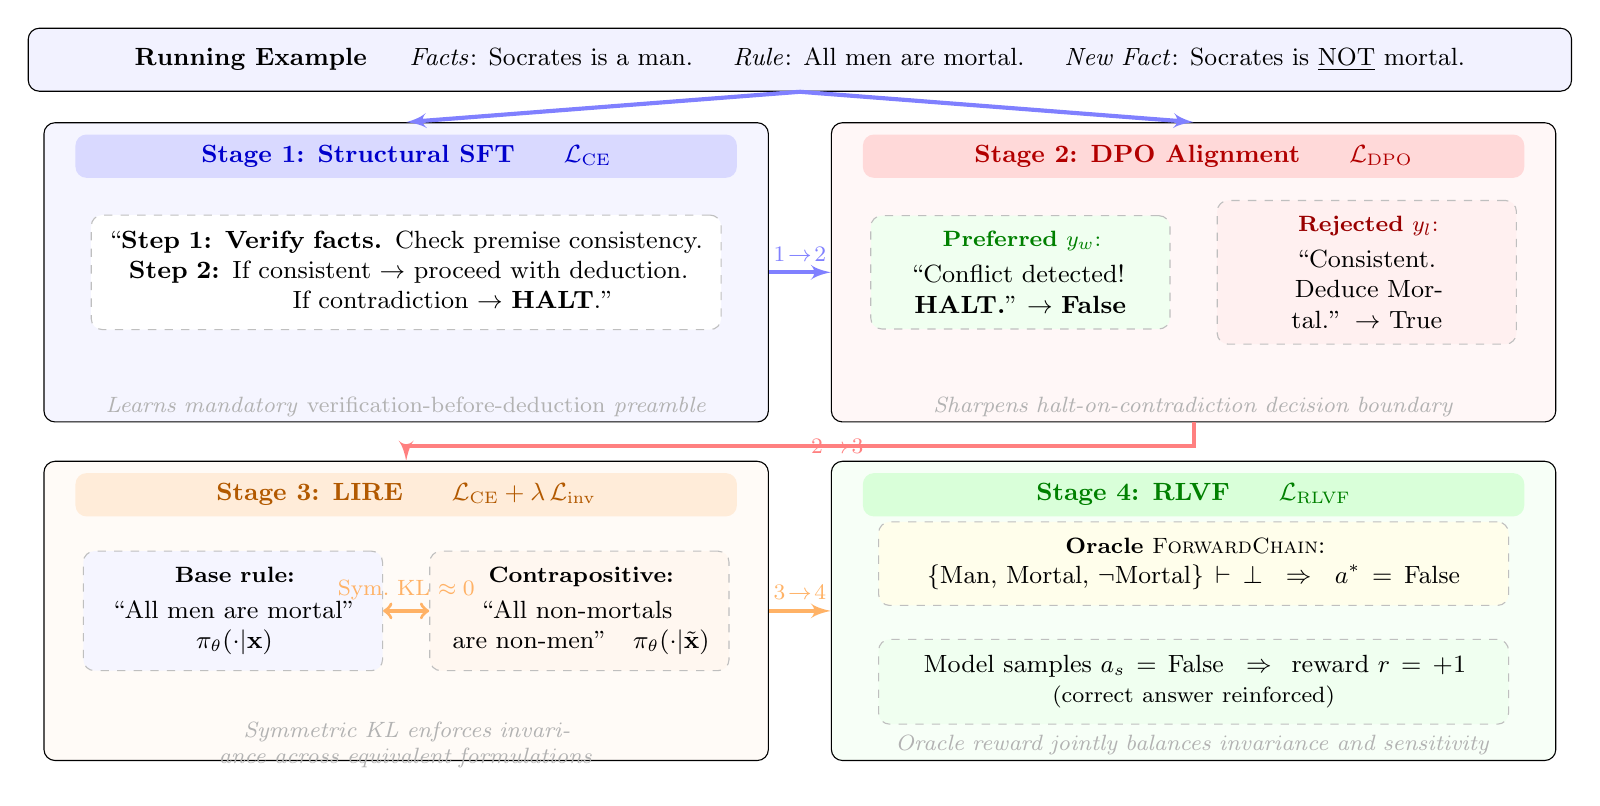
\begin{tikzpicture}
        % ── Styles ──────────────────────────────────────────
        \tikzstyle{sbox} = [rectangle, draw, rounded corners,
            minimum width=9.2cm, minimum height=3.8cm,
            inner sep=0.15cm]
        \tikzstyle{sheader} = [rectangle, rounded corners,
            minimum width=8.4cm, text centered, minimum height=0.55cm,
            font=\bfseries\small, anchor=north]
        \tikzstyle{scontent} = [rectangle, draw=gray!50, dashed, rounded corners,
            text width=7.6cm, text centered, font=\small,
            inner sep=0.2cm, fill=white]
        \tikzstyle{snote} = [font=\footnotesize\itshape, text=gray!60,
            text width=7.6cm, text centered]
        \tikzstyle{arr} = [draw, -latex', line width=1.5pt, >=stealth]
        \tikzstyle{inputbox} = [rectangle, draw, fill=blue!5,
            rounded corners, text centered, font=\small,
            minimum height=0.8cm]

        % ── Grid: cols at x=0,10; rows at y=0,-4.3 ─────────
        % Spacing tuned so input→top-row gap (~0.4cm) is slightly smaller
        % than top-row→bottom-row gap (~0.5cm) for visual balance.
        \def\colsep{10}
        \def\rowsep{-4.3}

        % ====================================================
        % INPUT — centered between the two columns
        % ====================================================
        \node [inputbox, minimum width=19.6cm] at (5, 2.7) (input) {
            \textbf{Running Example} ~~~
            \textit{Facts}: Socrates is a man. ~~
            \textit{Rule}: All men are mortal. ~~
            \textit{New Fact}: Socrates is \underline{NOT} mortal.
        };

        % ====================================================
        % STAGE 1: SFT  (top-left, x=0 y=0)
        % ====================================================
        \node [sbox, fill=blue!4] at (0, 0) (s1) {};
        % header: anchor=north so TOP edge starts 0.15cm below sbox top
        \node [sheader, fill=blue!15, text=blue!80!black]
              at ([yshift=-0.15cm]s1.north) (s1h)
              {Stage 1: Structural SFT ~~~ $\mathcal{L}_{\mathrm{CE}}$};
        \node [scontent] at (s1.center) (s1c) {
            ``\textbf{Step 1: Verify facts.} Check premise consistency. \\
            \textbf{Step 2:} If consistent $\to$ proceed with deduction. \\
            \phantom{Step 2:} If contradiction $\to$ \textbf{HALT}.''
        };
        \node [snote] at ([yshift=0.2cm]s1.south) (s1n) {
            Learns mandatory \emph{verification-before-deduction} preamble
        };

        % ====================================================
        % STAGE 2: DPO  (top-right, x=10 y=0)
        % ====================================================
        \node [sbox, fill=red!3] at (\colsep, 0) (s2) {};
        \node [sheader, fill=red!15, text=red!70!black]
              at ([yshift=-0.15cm]s2.north) (s2h)
              {Stage 2: DPO Alignment ~~~ $\mathcal{L}_{\mathrm{DPO}}$};
        \node [scontent, fill=green!6, text width=3.4cm]
              at ([xshift=-2.2cm]s2.center) (s2w) {
            {\footnotesize\color{green!50!black}\textbf{Preferred} $y_w$:} \\[2pt]
            ``Conflict detected! \\
            \textbf{HALT.}'' $\to$ \textbf{False}
        };
        \node [scontent, fill=red!6, text width=3.4cm]
              at ([xshift=2.2cm]s2.center) (s2l) {
            {\footnotesize\color{red!60!black}\textbf{Rejected} $y_l$:} \\[2pt]
            ``Consistent. \\
            Deduce Mortal.'' $\to$ True
        };
        \node [snote] at ([yshift=0.2cm]s2.south) (s2n) {
            Sharpens halt-on-contradiction decision boundary
        };

        % ====================================================
        % STAGE 3: LIRE  (bottom-left, x=0 y=-5)
        % ====================================================
        \node [sbox, fill=orange!3] at (0, \rowsep) (s3) {};
        \node [sheader, fill=orange!15, text=orange!70!black]
              at ([yshift=-0.15cm]s3.north) (s3h)
              {Stage 3: LIRE ~~~ $\mathcal{L}_{\mathrm{CE}} + \lambda\,\mathcal{L}_{\mathrm{inv}}$};
        \node [scontent, fill=blue!4, text width=3.4cm]
              at ([xshift=-2.2cm]s3.center) (s3a) {
            {\footnotesize \textbf{Base rule:}} \\[2pt]
            ``All men are mortal'' \\
            $\pi_\theta(\cdot|\mathbf{x})$
        };
        \node [scontent, fill=orange!6, text width=3.4cm]
              at ([xshift=2.2cm]s3.center) (s3b) {
            {\footnotesize \textbf{Contrapositive:}} \\[2pt]
            ``All non-mortals \\
            are non-men'' ~ $\pi_\theta(\cdot|\tilde{\mathbf{x}})$
        };
        \draw [<->, line width=1.2pt, orange!60] (s3a.east) -- (s3b.west)
              node[midway, above, font=\footnotesize] {Sym.\ KL $\approx 0$};
        \node [snote] at ([yshift=0.2cm]s3.south) (s3n) {
            Symmetric KL enforces invariance across equivalent formulations
        };

        % ====================================================
        % STAGE 4: RLVF  (bottom-right, x=10 y=-5)
        % ====================================================
        \node [sbox, fill=green!3] at (\colsep, \rowsep) (s4) {};
        \node [sheader, fill=green!15, text=green!50!black]
              at ([yshift=-0.15cm]s4.north) (s4h)
              {Stage 4: RLVF ~~~ $\mathcal{L}_{\mathrm{RLVF}}$};
        \node [scontent, fill=yellow!8]
              at ([yshift=0.6cm]s4.center) (s4c) {
            {\footnotesize \textbf{Oracle} \textsc{ForwardChain}}: \\
            $\{\text{Man},\, \text{Mortal},\, \neg\text{Mortal}\} \vdash \bot \;\Rightarrow\; a^* = \text{False}$
        };
        \node [scontent, fill=green!6]
              at ([yshift=-0.9cm]s4.center) (s4r) {
            Model samples $a_s = \text{False} \;\Rightarrow\;$ reward $r = +1$ \\
            {\footnotesize (correct answer reinforced)}
        };
        \node [snote] at ([yshift=0.2cm]s4.south) (s4n) {
            Oracle reward jointly balances invariance and sensitivity
        };

        % ====================================================
        % ARROWS
        % ====================================================
        % Input → top row (from input center down to each box top)
        \draw [arr, blue!50] (input.south) -- (s1.north);
        \draw [arr, blue!50] (input.south) -- (s2.north);

        % Z-flow: 1→2 (horizontal), 2→3 (diagonal), 3→4 (horizontal)
        \draw [arr, blue!50]   (s1.east) -- node[above, font=\footnotesize\bfseries] {$1 \!\to\! 2$} (s2.west);
        \draw [arr, red!50]    (s2.south) -- ++(0,-0.3) -| node[pos=0.25, right, font=\footnotesize\bfseries] {$2 \!\to\! 3$} (s3.north);
        \draw [arr, orange!60] (s3.east) -- node[above, font=\footnotesize\bfseries] {$3 \!\to\! 4$} (s4.west);

    \end{tikzpicture}%
    }% end resizebox
    \caption{Conflict-Aware Fusion on a running Socrates contradiction example. \textbf{Stage~1} (top-left, SFT) teaches the verification-before-deduction preamble and is the shared base; the other three panels are objectives trained \emph{from} it and compared, \textbf{not} a left-to-right chain. \textbf{DPO} (top-right) sharpens the halt boundary; \textbf{LIRE} (bottom-left) enforces output-distribution invariance via symmetric KL; \textbf{\textsc{RLVF}} (bottom-right), which produces our final model, uses a symbolic oracle reward and optimises invariance and sensitivity jointly.}
    \label{fig:fusion_structure}
\end{figure*}



\subsection{Retracted objectives: LIRE and DPO}
\label{app:retracted}
Retained verbatim from the earlier draft, for the record. The controls in
\S\ref{sec:v3control} and \S\ref{sec:shortcut} withdraw the claims made here:
LIRE's invariance gain is an artefact of all-True equivalence labels, and the
DPO branch cannot be measured on the generation path.

\paragraph{Why trace-level objectives are not enough.}
SFT and DPO both act on the reasoning \emph{trace}, and both leave \textit{surface-level pattern matching} intact: either can reach perfect accuracy on the original formulations yet drop sharply ($1.000 \to 0.327$ on De Morgan variants) once an equivalent rule is rephrased. The remaining two objectives act at the \emph{output-distribution} level instead.

\paragraph{Stage 3 (branch): Logical Invariance REgularisation (LIRE).}
Let $\mathbf{x}$ be a base premise-rule input, $\tilde{\mathbf{x}}$ its logically equivalent reformulation (De Morgan, double-negation, contrapositive), and $y=(y_1,\dots,y_T)$ the gold trace from the SFT data. LIRE penalises divergence between the next-token distributions under the two inputs, evaluated by \emph{teacher-forcing the same gold $y$} on both branches (which aligns the distributions token-wise and avoids variable-length rollout mismatch):
\begin{align}
\mathcal{L}_{\mathrm{LIRE}} &= \mathcal{L}_{\mathrm{CE}}\bigl(\pi_\theta(\cdot|\mathbf{x}),\, y\bigr) + \lambda\,\mathcal{L}_{\mathrm{inv}},\;\;
\mathcal{L}_{\mathrm{inv}} = \tfrac{1}{2 T}\!\sum_{t=1}^{T} \bigl[\mathrm{KL}_t(\mathbf{x}\Vert\tilde{\mathbf{x}}) + \mathrm{KL}_t(\tilde{\mathbf{x}}\Vert\mathbf{x})\bigr],
\label{eq:lire}
\end{align}
where $\mathrm{KL}_t(\mathbf{x}\Vert\tilde{\mathbf{x}}) := \mathrm{KL}\bigl(\pi_\theta(\cdot|\mathbf{x},y_{<t})\,\Vert\,\pi_\theta(\cdot|\tilde{\mathbf{x}},y_{<t})\bigr)$. Symmetry avoids the mode-seeking/covering asymmetry of unidirectional KL; the shared $y$ keeps the KL exact rather than approximated. This exactness carries a cost worth naming: teacher-forcing one gold trace on both branches presumes the two formulations admit derivations of the same length. For equivalence classes where they genuinely differ---a contrapositive rewrite introducing an extra negation-elimination step, say---the late-position KL measures ``how surprised is the policy, under the reformulated premises, that the \emph{original-form} continuation still holds'' rather than comparing two length-matched independent derivations. LIRE still measurably improves invariance (V4-multi $0.741\to0.999$), but it is an approximation with this specific, nameable failure mode.

\paragraph{Limitation of LIRE.}
LIRE improves invariance (Variant~4 accuracy $0.741 \to 0.999$) but suppresses \emph{any} distribution shift across rule reformulations, including those that \emph{should} change the answer (Variants~2/3): empirical sensitivity drops from $1.0$ to $0.47$. The invariance and sensitivity objectives are therefore in tension \emph{within a single loss}, which is what motivates replacing the regulariser with an oracle reward rather than stacking a fourth stage on top of it.



\subsection{Limitations and Future Work}
\label{app:limitations}

The benchmark is propositional and synthetic; saturation evidences that the structural prior \emph{generalises across backbones}, not that contradictions are universally solved---V4-multi at $1.5$B drops to $0.773$ after Stage~4 (a capacity bottleneck rather than a structural-prior failure; \S\ref{sec:phase2}), and the Lean F-rate gap on the closed-world / classical semantics divide is genuine. The pipeline also commits to a single \emph{conservative} contradiction semantics; paraconsistent or priority-based resolution strategies (Appendix~\ref{app:base-example} ff.) are out of scope. Three further limitations were surfaced in review and we state them explicitly. \textbf{(1)~External transfer is largely absent.} Zero-shot, every $1.5$B checkpoint collapses to a constant-\texttt{False} predictor on LogicNLI and MNLI, scoring exactly the majority-class baseline; the $8$B checkpoint collapses to constant-\texttt{True} on LogicNLI, scoring \emph{below} it; FOLIO at $8$B ($61.9\%$) is the only positive signal and ZebraLogic moves at neither scale (\S\ref{sec:external}). We therefore do not claim the prior escapes the synthetic template family. We also note a data-preparation defect we found and corrected: the released LogicNLI preparation script silently labelled all $500$ rows \texttt{False}, on which a constant-\texttt{False} predictor scores $1.000$; all figures reported here use labels rebuilt from the preserved \texttt{original\_label} field. \textbf{(2)~Oracle/label coupling in Phase~1.} The \textsc{RLVF} reward is the same forward-chaining engine that defines the benchmark labels. This is true by construction in the propositional regime and is a property of Phase~1, not a claim that \textsc{RLVF} works detached from a ground-truth source; it is precisely why Phase~2 replaces the oracle with an externally specified Lean~4 kernel (\S\ref{sec:phase2}). \textbf{(3)~LIRE's length assumption.} Teacher-forcing a shared gold trace presumes length-matched derivations across equivalent formulations, which some rewrites violate (\S\ref{sec:pipeline}). Three concrete next steps follow: (i) end-to-end RLVF-Lean training amortised through a persistent LeanDojo server, replacing the current verification-only deployment; (ii) lifting the closed-world override via a CWA axiom schema, or via the hybrid forward-chain/Lean policy of \S\ref{sec:phase2} that uses Lean only for T-verdicts and the symbolic forward-chainer for F-verdicts; (iii) evaluation on math/proof benchmarks (e.g., MiniF2F, ProofNet) where the Lean kernel is the natural verifier and where stacked-rewrite depth substantially exceeds the $2$--$5$ laws stress-tested in V4-multi.

\subsection{Qualitative Analysis: Why Frontier Models Fail}
\label{app:qualitative}
To understand the failure mode of frontier models, we performed an error analysis on GPT-4o using the OpenAI API on a stratified $200$-row sample per split (the per-question prediction CSVs are released alongside the benchmark). On Variant~3, where every query has ground-truth \texttt{False} under conservative reasoning semantics, GPT-4o produces the correct halt-on-contradiction answer in only $56.0\%$ of the $800$ test questions; the remaining $44.0\%$ continue deductive inference despite the explicit contradiction in the premises. A representative failure: given premises $\{A \to B,\, A,\, \neg B\}$, GPT-4o often surfaces the inconsistency in its verification trace and then proceeds to conclude $B$ from $\{A \to B, A\}$, stating ``Since $A$ is true and $A$ implies $B$, then $B$ must be true,'' effectively ignoring its own prior verification of $\neg B$. This suggests that frontier models suffer from a compartmentalization of verification and execution, where the ``reasoning momentum'' of the deductive steps overrides contradictory evidence. To rule out a vendor-specific artefact, we replicate the analysis on \textbf{Gemma-3-4B-IT} (an open-weight frontier model from a different lab, evaluated locally with identical prompts and decoding); it scores \emph{lower} on V3 ($0.439$) than GPT-4o, continuing past the contradiction in $56.1\%$ of cases, and shows the same qualitative failure pattern. Fusion-Conflict mitigates this by fusing the verification signal directly into the hidden state representation, forcing the model to reconcile the conflict before proceeding.


\subsection{Baseline Failure Pattern Across Backbones}
\label{app:baseline-table}

\begin{table*}[t]
\centering
\small
\begin{tabular}{lcccccc}
\toprule
& \multicolumn{2}{c}{\textbf{BERT}} &
  \multicolumn{2}{c}{\textbf{Qwen2}} &
  \multicolumn{2}{c}{\textbf{TinyLlama}} \\
\cmidrule(lr){2-3} \cmidrule(lr){4-5} \cmidrule(lr){6-7}
\textbf{Split} & Acc & $\Delta$ & Acc & $\Delta$ & Acc & $\Delta$ \\
\midrule
base                            & 1.0000 & 0.0000 & 1.0000 & 0.0000 & 1.0000 & 0.0000 \\
variant1                        & 1.0000 & 0.0000 & 1.0000 & 0.0000 & 1.0000 & 0.0000 \\
variant2 (Essential Deletion)   & 0.2950 & -0.7050 & 0.2500 & -0.7500 & 0.2500 & -0.7500 \\
variant3 (Contradiction)        & 0.0000 & -1.0000 & 0.0000 & -1.0000 & 0.0000 & -1.0000 \\
variant4-multi (Stacked Laws)   & 1.0000 & 0.0000 & 0.6450 & -0.3550 & 0.9925 & -0.0075 \\
\bottomrule
\end{tabular}
\caption{Baseline Performance: Accuracy and deviation ($\Delta$) across structural variants without fusion optimization.}
\label{tab:all_models_deltas}
\end{table*}


\subsection{Lean~4 Benchmark-Scale Verification: Per-Split Breakdown}
\label{app:lean-bench-table}

\begin{table}[h]
\centering
\small
\caption{Lean~4 verification on LEMO benchmark rows ($20$ rows per split, stratified; $187$ questions). \textbf{Polarity is each query's \emph{classical} label}---derivable from the premises \emph{before} the conservative-semantics override of \S\ref{sec:method}---not the per-instance ``everything-is-\texttt{F}'' override applied to Variant~3 elsewhere; this is why Variant~3 still contains $12$ classically-derivable T-cases, and why the table tests whether Lean can perform the derivation rather than whether it reproduces the override. Variant~1 draws all-T queries because removing \emph{redundant} rules preserves derivability of the original T-queries, so the stratified $20$-row draw contained $42$ T- and zero F-queries. The T/F gap is analysed below.}
\label{tab:lean_bench}
\begin{tabular}{lrrrrrr}
\toprule
& \multicolumn{3}{c}{\textbf{Ground truth = T}} & \multicolumn{3}{c}{\textbf{Ground truth = F}} \\
\cmidrule(lr){2-4} \cmidrule(lr){5-7}
\textbf{Split} & \textbf{\#T} & \textbf{Accept} & \textbf{Rate} & \textbf{\#F} & \textbf{Accept} & \textbf{Rate} \\
\midrule
base                         & 29  & 28  & $96.6\%$ & 32  & 12 & $37.5\%$ \\
variant1 (redundant removal) & 42  & 42  & $100.0\%$ & 0   & 0  & --- \\
variant2 (essential removal) & 22  & 22  & $100.0\%$ & 20  & 0  & $0.0\%$ \\
variant3 (contradiction)     & 12  & 12  & $100.0\%$ & 30  & 18 & $60.0\%$ \\
\midrule
\textbf{Overall}             & \textbf{105} & \textbf{104} & \textbf{99.0\%} & \textbf{82} & \textbf{30} & \textbf{36.6\%} \\
\bottomrule
\end{tabular}
\end{table}


\subsection{Why Plain REINFORCE Suffices for \textsc{RLVF}}
\label{app:reinforce}
\label{app:rlvf-rationale}

We initially gave three reasons why plain REINFORCE should suffice: a
deterministic $\pm1$ reward has low gradient variance, the EMA baseline already
removes the running mean, and the oracle offers no reward-hacking surface.
Only the third survives. Without a trust region the EMA baseline climbed to
$+0.695$, making a wrong trace $5.6\times$ more costly than a correct one was
valuable, and the policy collapsed into non-parsing output at step~$250$; a KL
penalty against the initialisation was required to train the full $600$ steps.
A deterministic reward bounds bias, not estimator variance. Separately, an
outcome-only reward cannot distinguish detecting a contradiction from answering
False unconditionally---both earn the same return---so it is degenerate for
this capability regardless of the optimiser (Table~\ref{tab:v3control}).

\subsection{Compute Footprint per Stage}
\label{app:compute}

Table~\ref{tab:compute} reports measured wall-clock time per stage, taken from the
training logs of the exact checkpoints released with the code
(\texttt{trained\_models/qwen}, \texttt{qwen\_lire}, \texttt{qwen\_rlvf} and their
Qwen3-8B counterparts), so each row is traceable to a specific run rather than an
estimate. The whole pipeline is a few GPU-hours on a single device; the dominant
cost at $8$B is Stage~4, whose rollouts are generation-bound rather than
gradient-bound. Dataset construction adds no annotation cost: the generator is
template-driven and combinatorial (Appendix~\ref{app:variant-gen}), so scaling to
more base groups means increasing $N$ in the generator, not hiring annotators.

\begin{table}[h]
\centering\small
\caption{Measured wall-clock training time per stage on a single GPU (LoRA $+$ bf16), read from the released training logs. Because the objectives are branches off one base (\S\ref{sec:pipeline}), the released model costs only Stage~1~$+$~Stage~4; the DPO and LIRE branches are additional runs used for the comparisons in Tables~\ref{tab:comparison_results} and~\ref{tab:stage_wise}, not prerequisites. The Qwen3-8B Stage-1 run is a short $180$-step LoRA pass. Lean kernel verification (Phase~2) is a separate $\sim\!0.36$\,s/trace CPU cost incurred only during training.}
\label{tab:compute}
\begin{tabular}{lcc}
\toprule
\textbf{Stage} & \textbf{Qwen2-1.5B} & \textbf{Qwen3-8B} \\
\midrule
Stage 1 --- Structural SFT (shared base)  & $4.15$\,h & $0.02$\,h \\
Stage 4 --- \textsc{RLVF} (final model)   & $0.94$\,h & $9.69$\,h \\
\midrule
\textbf{Cost of the released model}       & $\mathbf{5.09}$\,\textbf{h} & $\mathbf{9.71}$\,\textbf{h} \\
\midrule
Stage 2 --- DPO branch (comparison only)  & $0.90$\,h & --- \\
Stage 3 --- LIRE branch (comparison only) & $1.26$\,h & $4.26$\,h \\
\bottomrule
\end{tabular}
\end{table}

\subsection{LEMO-to-Lean Translation}
\label{app:lean-translator}

Section~\ref{sec:phase2} evaluates a Lean~4 kernel against benchmark instances translated automatically from our CSV schema. The translator (\texttt{lean\_demo/lemo\_to\_lean.py}) is deliberately small and total on the benchmark's surface grammar; we specify it here so the Lean results are independently reproducible.

\begin{enumerate}
\item \textbf{Parse.} Each fact, rule, and question is matched against a closed set of natural-language templates: positive facts (\emph{``$X$ is $P$''}), disjunctive facts (\emph{``$X$ is $P$ or $Q$''}), negated facts (\emph{``$X$ is not $P$''}), rules of the form \emph{``If something is $P$ then something is $Q$''}, and their negated variants. Any instance containing a string outside this grammar is rejected rather than silently mistranslated.
\item \textbf{Declare.} Every distinct predicate occurring anywhere in the instance is declared as a Lean \texttt{Prop}. The benchmark is propositional, so no quantifier machinery is emitted.
\item \textbf{Emit hypotheses.} Facts and rules become hypotheses of the generated theorem. Disjunctive facts are discharged by $\lor$-elimination, producing one branch per disjunct.
\item \textbf{Emit theorem and proof skeleton.} For each question the translator emits a theorem statement encoding the expected answer, together with a proof script of chained \texttt{have} statements mirroring the steps of the symbolic forward-chaining oracle. The oracle is therefore reused to produce the \emph{proof skeleton}, not merely the label---which is what makes the kernel's verdict a check on the derivation rather than on the answer.
\item \textbf{Dispatch.} The generated \texttt{.lean} file is compiled by the \texttt{lean} kernel and the accept/reject verdict recorded. A worked multi-step example beyond the toy Socrates case is included in the released code alongside the generated \texttt{.lean} artefacts.
\end{enumerate}

Two consequences are worth stating. First, the kernel arbitrates \emph{classical} derivability, which is why Table~\ref{tab:lean_bench} is scored against classical (pre-override) polarities rather than the conservative instance labels. Second, the rejection-on-unparsed policy means kernel agreement is a lower bound restricted to instances the translator fully covers, not an average over silently degraded translations.

\subsection{Structural Variant Generation}
\label{app:variant-gen}

\begin{algorithm}[h]
\caption{Structural Variant Generation (Variant 2 \& 3)}
\label{alg:variant23}
\small
\begin{algorithmic}[1]
\Require Canonical generator $\mathsf{Base}(\cdot)$, key rule $r^\star$, contradiction template $\mathsf{Contr}(\cdot)$, instances $N$
\Ensure Datasets $\mathcal{D}_{base}, \mathcal{D}_{v2}, \mathcal{D}_{v3}$
\For{$i=1$ to $N$}
    \State $(F,R,Q,A) \gets \mathsf{Base}(i)$;\quad $\mathcal{D}_{base} \gets \mathcal{D}_{base} \cup \{(F,R,Q,A)\}$
    \State $R_{v2} \gets R \setminus \{r^\star\}$;\quad $\mathcal{D}_{v2} \gets \mathcal{D}_{v2} \cup \{(F,R_{v2},Q,\mathsf{Label}(F,R_{v2},Q))\}$
    \State $F_{v3} \gets F \cup \{\mathsf{Contr}(F,R)\}$;\quad $\mathcal{D}_{v3} \gets \mathcal{D}_{v3} \cup \{(F_{v3},R,Q,\mathsf{Label}(F_{v3},R,Q))\}$
\EndFor
\end{algorithmic}
\end{algorithm}

\subsection{Preference Pair Templates (DPO Stage 2)}
\label{app:pref-pairs}
For contradiction cases, the preferred reasoning trace $y_w$ correctly detects the inconsistency in the verification step and halts; the rejected trace $y_l$ proceeds with deductive inference.

\textbf{Preferred ($y_w$):}~``Step 1: Detect contradiction between premises. Step 2: Halt reasoning.''\quad
\textbf{Rejected ($y_l$):}~``Step 1: Premises are consistent. Step 2: Continue deductive inference.''

\subsection{Stage 1 Hyperparameters}
\label{app:hyper}
Epochs $3$; LR $2{\times}10^{-5}$; batch $4$; max length $512$; AdamW (mixed precision); LoRA $r{=}8$, $\alpha{=}16$, dropout $0.05$.

\subsection{Stage-wise objective comparison (legacy figures)}
\label{app:stagewise}
These figures were measured before the benchmark was regenerated on
2026-03-31 and have not been re-verified against the current data; they
are retained for continuity with the earlier draft and are not used to
support any claim in the main text.

\begin{table}[h]
\centering\small
\caption{Objective comparison over a shared Stage-1 base. \textbf{Branches, not a chain}: rows~2 and~3 are each trained from the row-1 checkpoint (\S\ref{sec:pipeline}). LIRE buys compositional invariance but \emph{collapses} V2/V3 sensitivity; \textsc{RLVF}, from the same base and drawing half of each batch from the same invariance pairs, reaches oracle-level V2/V3 \emph{and} most of the V4 gain in one run. At $1.5$B it retains $0.773$ on V4-multi against LIRE's $0.993$---a residual we report rather than claim ``no loss''; at $8$B it matches the LIRE ceiling. Row~1 is the Stage-1 SFT checkpoint, \emph{not} an untrained zero-shot run and with no preference optimisation applied; DPO is a separate branch, evaluated in Table~\ref{tab:comparison_results}.}
\label{tab:stage_wise}
\begin{tabular}{l|cccc|cccc}
\toprule
& \multicolumn{4}{c|}{\textbf{Qwen2-1.5B}} & \multicolumn{4}{c}{\textbf{Qwen3-8B}} \\
\textbf{Stage}            & Base & V2   & V3   & V4-multi & Base & V2   & V3   & V4-multi \\
\midrule
SFT (Stage~1)             & $1.000$ & $1.000$ & $1.000$ & $0.635$  & $0.333$ & $0.460$ & $0.656$ & $0.006$  \\
SFT $\to$ LIRE (Stage~3)  & $0.812$ & $0.590$ & $0.344$ & $\mathbf{0.993}$ & $0.549$ & $0.503$ & $0.344$ & $\mathbf{1.000}$ \\
SFT $\to$ \textsc{RLVF} (St.~4) & $\mathbf{1.000}$ & $\mathbf{1.000}$ & $\mathbf{1.000}$ & $0.773$ & $\mathbf{1.000}$ & $\mathbf{1.000}$ & $\mathbf{1.000}$ & $\mathbf{1.000}$ \\
\bottomrule
\end{tabular}
\end{table}

\subsection{Ablation Tables}
\label{app:ablation}

\begin{table}[h]
\centering\small
\caption{Ablation: SFT on a vanilla \emph{Mixed-Aug} corpus \emph{without} the conflict-aware verification preamble. Compared to Fusion-LRA (Conflict-Aware SFT, Table~\ref{tab:comparison_results}, Base $=0.988$ on Qwen2), removing the preamble drops Qwen2's base accuracy to $0.5250$, isolating the contribution of the structural prior from the contribution of training data alone.}
\label{tab:stage1_results}
\begin{tabular}{lcccccc}
\toprule
& \multicolumn{2}{c}{\textbf{BERT}} & \multicolumn{2}{c}{\textbf{Qwen2}} & \multicolumn{2}{c}{\textbf{TinyLlama}} \\
\cmidrule(lr){2-3}\cmidrule(lr){4-5}\cmidrule(lr){6-7}
\textbf{Split} & Acc & $\Delta$ & Acc & $\Delta$ & Acc & $\Delta$ \\
\midrule
base                            & 1.0000 & 0.0000 & 0.5250 & -0.4750 & 0.5375 & -0.4625 \\
variant2 (Essential Deletion)   & 0.2500 & -0.7500 & 0.4050 & -0.1200 & 0.5325 & -0.0050 \\
variant3 (Contradiction)        & 0.0000 & -1.0000 & 0.0000 & -1.0000 & 0.0000 & -1.0000 \\
\bottomrule
\end{tabular}
\end{table}

\begin{table}[h]
\centering\small
\caption{Iterative Comparison: Fusion-LRA vs.\ earlier iterations.}
\label{tab:final_performance_comparison}
\begin{tabular}{lcccc}
\toprule
\textbf{Method} & \textbf{Base Acc} & \textbf{Var 2} & \textbf{Var 3} & \textbf{Rank} \\
\midrule
Mixed-Aug              & 0.525          & 0.405          & 0.972          & 3 \\
RA-CoT                 & 0.263          & 0.593          & 0.690          & 2 \\
\midrule
\textbf{Fusion-LRA}    & \textbf{0.988} & \textbf{0.753} & 0.705          & \textbf{1} \\
\bottomrule
\end{tabular}
\end{table}

\subsection{Lean Pilot Study (8 hand-crafted traces)}
\label{app:lean-pilot-note}
One non-trivial engineering finding: Lean's \texttt{sorry} exits with status~0, so the bridge must treat \texttt{sorry}/\texttt{admit} as $-1$ rather than trusting the exit code. Production deployment would amortise dispatch via a \textsc{LeanDojo}~\citep{yang2023leandojo} persistent server. Lean complements \textsc{ForwardChain} in expressiveness (quantifiers and induction vs.\ Horn clauses), granularity (per-tactic verdicts), and compositionality, and is feasible end-to-end given recent neural theorem proving~\citep{yang2023leandojo,polu2020gpt-f,alphaproof2024}.

\label{app:lean-pilot}

Before the benchmark-scale Lean evaluation reported in Table~\ref{tab:lean_bench}, we ran a small hand-crafted pilot on the Socrates contradiction example to verify (i)~that the Python$\to$Lean bridge faithfully translates a halt-on-contradiction trace into a kernel-checkable theorem, (ii)~that valid halt traces receive reward~$+1$ while opportunistic deductive continuations and malformed traces receive $-1$, and (iii)~that per-trace verification latency is compatible with online RL. Table~\ref{tab:lean_pilot} reports kernel agreement on $8$ representative traces.

\begin{table}[h]
\centering\small
\caption{Lean~4 step-level reward pilot on the Socrates example. Lean kernel agrees with the expected RLVF-Lean reward on $8/8$ traces, including \texttt{sorry}-based admits and syntactic errors. Mean latency $0.36$\,s/trace on CPU.}
\label{tab:lean_pilot}
\begin{tabular}{llrrr}
\toprule
\textbf{Trace ID} & \textbf{Category} & \textbf{Expected $r$} & \textbf{Lean $r$} & \textbf{Time (s)} \\
\midrule
T1-halt-minimal              & correct halt       & $+1$ & $+1$ & 0.36 \\
T2-halt-direct               & correct halt       & $+1$ & $+1$ & 0.38 \\
T3-halt-contradiction-tactic & correct halt       & $+1$ & $+1$ & 0.36 \\
T4-naive-stops-early         & na\"ive continue   & $-1$ & $-1$ & 0.37 \\
T5-naive-wrong-goal          & na\"ive continue   & $-1$ & $-1$ & 0.35 \\
T6-naive-empty (\texttt{sorry}) & na\"ive continue & $-1$ & $-1$ & 0.36 \\
T7-syntax-error              & malformed          & $-1$ & $-1$ & 0.36 \\
T8-misspelled-lemma          & malformed          & $-1$ & $-1$ & 0.36 \\
\midrule
\multicolumn{2}{l}{\textbf{Agreement with oracle}} & \multicolumn{3}{r}{\textbf{8/8 (100\%)}} \\
\bottomrule
\end{tabular}
\end{table}

\subsection{Lean 4 Feasibility Demo for RLVF-Lean (Phase 2)}
\label{app:lean-demo}

The following Lean~4 script encodes the Socrates contradiction example from
Figure~\ref{fig:fusion_structure} as a verified theorem. It accompanies
Section~\ref{sec:phase2} (\emph{Phase 2: Scaling the Verifier with a Formal
Proof Assistant}) and demonstrates that the step-level reward signal defined
by the step-level reward of \S\ref{sec:phase2} can be sourced from the Lean kernel with no
additional model training. The complete source is included in
\texttt{lean\_demo/SocratesContradiction.lean}; a minimal excerpt is shown
below.

\begin{verbatim}
axiom Person   : Type
axiom Socrates : Person
axiom Man      : Person -> Prop
axiom Mortal   : Person -> Prop
axiom men_are_mortal : forall x : Person, Man x -> Mortal x

-- The halt-on-contradiction behavior that RLVF-Lean is rewarded
-- for discovering. Lean accepts the proof iff the policy has
-- genuinely identified both sides of the contradiction.
theorem socrates_contradiction
    (h_man        : Man Socrates)
    (h_not_mortal : Not (Mortal Socrates)) : False := by
  have h_mortal : Mortal Socrates := men_are_mortal Socrates h_man
  exact absurd h_mortal h_not_mortal
\end{verbatim}

A Python bridge (\texttt{lean\_demo/lean\_verifier\_bridge.py}) synthesizes
one such script per policy rollout and returns the kernel's accept/reject
verdict as the step-level reward $r_t$ of \S\ref{sec:phase2}. The
same theorem additionally refutes the naive ``continue deducing'' policy:
under the contradictory premise set, no total proof of an arbitrary query
exists without first deriving \texttt{False}, so any rollout that claims
\texttt{True} receives reward~$-1$. This preserves the conservative
reasoning semantics of Section~\ref{sec:method} at the level of the Lean
kernel itself.

\subsection{Base Example: Complex Dilemma Reasoning Structure}
\label{app:base-example}
We begin with a comprehensive example that establishes the core reasoning pattern, drawing on a structure analogous to the \textit{Paradox of the Court}\footnote{The Paradox of the Court involves a contract between the teacher Protagoras and his student Euathlus, where the student only pays for lessons if he wins a court case. When Protagoras sues Euathlus for the fee, a paradox arises: if Euathlus wins, he owes nothing, but if he loses, he still avoids payment, creating a logical contradiction about the outcome.}, a classic logical dilemma where multiple possible paths lead to the same conclusion, despite their apparent differences.

\begin{itemize}
    \item \textbf{Facts:}
    \begin{itemize}
        %\item Anne is a person
        \item Anne is green or blue
        %\item Anne is not cold or not nice [contradiction fact]
    \end{itemize}

    \item \textbf{Rules:}
    \begin{itemize}
        \item Rule 1: If someone is green then they are cold. $\forall x \, (\text{Green}(x) \rightarrow \text{Cold}(x))$
        \item Rule 2: If someone is blue then they are cold. $\forall x \, (\text{Blue}(x) \rightarrow \text{Cold}(x))$
        \item Rule 3: If someone is cold then they are rough. $\forall x \, (\text{Cold}(x) \rightarrow \text{Rough}(x))$
        \item Rule 4: If someone is rough then they are young. $\forall x \, (\text{Rough}(x) \rightarrow \text{Young}(x))$
        \item Rule 5: If someone is young then they are cold. $\forall x \, (\text{Young}(x) \rightarrow \text{Cold}(x))$
        \item Rule 6: If someone is young then they are nice. $\forall x \, (\text{Young}(x) \rightarrow \text{Nice}(x))$
        %\item $(\neg p \rightarrow \neg r)\wedge (\neg q \rightarrow \neg r)\wedge (\neg p \vee \neg q)\vdash \neg r $
    \end{itemize}

    \item \textbf{Questions:}
    \begin{itemize}
        \item Q1: Anne is cold. True/False? [Answer: T]
        \item Q2: Anne is rough. True/False? [Answer: T]
        \item Q3: Anne is young. True/False? [Answer: T]
        \item Q4: Anne is nice. True/False? [Answer: T]
    \end{itemize}
\end{itemize}

The fact ``Anne is green or blue" combined with Rules 1 and 2 creates a classic dilemma: both possibilities lead to the same conclusion. This dilemma reasoning yields  ``Anne is cold." Rule 3 then derives ``Anne is rough" from cold, Rule 4 derives ``Anne is young" from rough, and Rule 6 derives ``Anne is nice" from young. Rule 5 creates a circular reinforcement but doesn't alter the conclusions.

The logical structure can be represented as:
\[
(G_a \lor B_a) \land (G_a \rightarrow C_a) \land (B_a \rightarrow C_a) \vdash C_a
\]

\begin{itemize}
    \item $G_a$: \text{Green}(Anne)
    \item $B_a$: \text{Blue}(Anne)
    \item $C_a$: \text{Cold}(Anne)
\end{itemize}


\subsection{Variation 1: Rule Reduction with Same Conclusions}

This variation demonstrates that removing redundant rules preserves the AI's ability to reach the same conclusions, illustrating that fewer rules can be equally effective.

\begin{itemize}
    \item \textbf{Facts:}
    \begin{itemize}
        \item Anne is green or blue
    \end{itemize}

    \item \textbf{Rules:}
    \begin{itemize}
        \item Rule 1: If someone is green then they are cold. $\forall x \, (\text{Green}(x) \rightarrow \text{Cold}(x))$
        \item Rule 2: If someone is blue then they are cold. $\forall x \, (\text{Blue}(x) \rightarrow \text{Cold}(x))$
        \item Rule 3: If someone is cold then they are rough. $\forall x \, (\text{Cold}(x) \rightarrow \text{Rough}(x))$
        \item Rule 4: If someone is rough then they are young. $\forall x \, (\text{Rough}(x) \rightarrow \text{Young}(x))$
        \item Rule 6: If someone is young then they are nice. $\forall x \, (\text{Young}(x) \rightarrow \text{Nice}(x))$
        % Rule 5 removed - redundant
    \end{itemize}

    \item \textbf{Questions:}
    \begin{itemize}
        \item Q1: Anne is cold. True/False? [Answer: T]
        \item Q2: Anne is rough. True/False? [Answer: T]
        \item Q3: Anne is young. True/False? [Answer: T]
        \item Q4: Anne is nice. True/False? [Answer: T]
    \end{itemize}
\end{itemize}

The reasoning proceeds identically to the base case: the dilemma from Rules 1-2 yields ``Anne is cold," Rule 3 yields rough, Rule 4 yields young, and Rule 6 yields nice. The removal of Rule 5 has no impact on the conclusions, demonstrating its redundancy.

\textbf{Key Insight}: AI systems that recognize this redundancy can simplify their reasoning processes without sacrificing accuracy, embodying the ``less is more" principle.

The simplified logical structure becomes:
\[
(G_a \lor B_a) \land (G_a \rightarrow C_a) \land (B_a \rightarrow C_a) \vdash C_a
\]

\[
C_a \land (C_a \rightarrow R_a) \vdash R_a
\]


\[
R_a \land (R_a \rightarrow Y_a) \vdash Y_a
\]


\[
Y_a \land (Y_a \rightarrow N_a) \vdash N_a
\]

\begin{itemize}
    \item $G_a = \mathrm{Green}(Anne)$
    \item $B_a = \mathrm{Blue}(Anne)$
    \item $C_a = \mathrm{Cold}(Anne)$
    \item $R_a = \mathrm{Rough}(Anne)$
    \item $Y_a = \mathrm{Young}(Anne)$
    \item $N_a = \mathrm{Nice}(Anne)$
\end{itemize}


\subsection{Variation 2: Rule Equivalence with Different Conclusions}

This variation replaces multiple rules with logically equivalent fewer rules, but interestingly leads to different conclusions due to the modified rule interactions.

\begin{itemize}
    \item \textbf{Facts:}
    \begin{itemize}
        %\item Anne is a person
        \item Anne is green or blue
    \end{itemize}

    \item \textbf{Rules:} (\emph{This variant deliberately combines two perturbations: a logical-equivalence rewrite of Rules~1+2 into a single Rule~A, \textbf{and} the deletion of Rules~5 and~6. Rule~6 is essential for deriving ``nice''; we discuss the two perturbations separately below.})
    \begin{itemize}
        \item Rule A: If someone is green or blue then they are cold. $\forall x \, ((\text{Green}(x) \lor \text{Blue}(x)) \rightarrow \text{Cold}(x))$ \quad \emph{(replaces Rules 1+2)}
        \item Rule 3: If someone is cold then they are rough. $\forall x \, (\text{Cold}(x) \rightarrow \text{Rough}(x))$
        \item Rule 4: If someone is rough then they are young. $\forall x \, (\text{Rough}(x) \rightarrow \text{Young}(x))$
        \item \emph{Rule~5 (Young $\to$ Cold) -- removed (redundant cycle)}
        \item \emph{Rule~6 (Young $\to$ Nice) -- removed (essential for ``nice''; this is the cause of Q4=F, not the Rule~A rewrite)}
    \end{itemize}

    \item \textbf{Questions:}
    \begin{itemize}
        \item Q1: Anne is cold. True/False? [Answer: T]
        \item Q2: Anne is rough. True/False? [Answer: T]
        \item Q3: Anne is young. True/False? [Answer: T]
        \item Q4: Anne is nice. True/False? [Answer: F]
    \end{itemize}
\end{itemize}

Rule~A directly captures the dilemma of Rules 1 and 2, leading to ``Anne is cold" with equivalent logical force---this is the equivalence rewrite, and it preserves Q1--Q3. The change in Q4 (``nice'' becomes F) is caused entirely by the \emph{deletion of Rule~6}, not by the equivalence rewrite. We made both edits in this single illustrative variant to keep the example compact, but they are structurally independent: Variant~4 in the main benchmark applies the rewrite alone, and Variant~2 applies the essential-rule deletion alone.

\textbf{Key Insight}: Logical equivalence of a sub-rule set (here Rules~1+2 vs.\ Rule~A) is a local property; it does not by itself change derivability. Macro-level derivability changes are caused by which essential rules remain, as isolated cleanly in Variant~2.

The logical equivalence can be shown as:
\[
(\forall x \, (G_x \rightarrow C_x) \land \forall x \, (B_x \rightarrow C_x))
\equiv
\forall x \, ((G_x \lor B_x) \rightarrow C_x)
\]

\begin{itemize}
    \item $G_x = \mathrm{Green}(x)$
    \item $B_x = \mathrm{Blue}(x)$
    \item $C_x = \mathrm{Cold}(x)$
\end{itemize}


However, the missing Rule 6 prevents the derivation of Nice(Anne), showing that local equivalence doesn't preserve global derivability.

\subsection{Variation 3: Rule Interference with Contradictory Conclusions}

This variation adds distracting and potentially contradictory rules, testing the AI's ability to address conflicts and maintain coherent reasoning.

\begin{itemize}
    \item \textbf{Facts:}
    \begin{itemize}
        %\item Anne is a person
        \item Anne is green or blue
        \item Anne is not cold or not nice
    \end{itemize}

    \item \textbf{Rules:}
    \begin{itemize}
        \item Rule 1: If someone is green then they are cold. $\forall x \, (\text{Green}(x) \rightarrow \text{Cold}(x))$
        \item Rule 2: If someone is blue then they are cold. $\forall x \, (\text{Blue}(x) \rightarrow \text{Cold}(x))$
        \item Rule 3: If someone is cold then they are rough. $\forall x \, (\text{Cold}(x) \rightarrow \text{Rough}(x))$
        \item Rule 4: If someone is rough then they are young. $\forall x \, (\text{Rough}(x) \rightarrow \text{Young}(x))$
        \item Rule 5: If someone is young then they are cold. $\forall x \, (\text{Young}(x) \rightarrow \text{Cold}(x))$
        \item Rule 6: If someone is young then they are nice. $\forall x \, (\text{Young}(x) \rightarrow \text{Nice}(x))$
        %\item Rule 7: If someone is nice then they are not cold. $\forall x \, (\text{Nice}(x) \rightarrow \neg \text{Cold}(x))$ \quad \text{//

    \end{itemize}

    \item \textbf{Questions:}
    \begin{itemize}
        \item Q1: Anne is cold. True/False? [Answer: F]
        \item Q2: Anne is rough. True/False? [Answer: F]
        \item Q3: Anne is young. True/False? [Answer: F]
        \item Q4: Anne is nice. True/False? [Answer: F]
    \end{itemize}
\end{itemize}


\subsection{Reasoning Process and Analysis}

    This variation introduces \textit{contradictory interference}, which challenges the AI's ability to address conflicts within the logical structure. The fact ``Anne is green or blue," combined with the original chain of reasoning (Rules 1-6), leads to the conclusions that Anne is cold, rough, young, and nice. However, the fact ``Anne is not cold or not nice" introduces a conflict, as it implies that being nice would mean Anne is not cold. This creates a contradiction that different AI systems might address differently:

\paragraph{Contradiction Handling Strategy.}

In the experiments presented in this paper we adopt a \textit{conservative}
contradiction-handling strategy. Once a contradiction is detected in the
premise set, the reasoning process halts and no further deductions are
performed. As a result, all queries associated with that instance are
labeled \texttt{False}.

Alternative reasoning strategies such as priority-based resolution or
paraconsistent reasoning are possible, but they are outside the scope
of the current work and are left for future investigation.

\begin{itemize}
    \item \textbf{Conservative approach}: Detect contradiction and withhold conclusions
    \item \textbf{Priority-based approach}: Apply rule priorities or specificity heuristics
    \item \textbf{Paraconsistent approach}: Accept some contradictions and continue reasoning
\end{itemize}

In this case, a conservative reasoning system would recognize the contradiction and potentially reject all derived conclusions, resulting in \textit{false} for all questions.

 The addition of interfering rules not only tests the AI's ability to ignore distractions but also its capacity for contradiction detection and resolution.

The contradiction can be formally represented as:
\[
(C_a \land N_a) \land (N_a \rightarrow \neg C_a) \vdash \bot
\]

\begin{itemize}
    \item $C_a = \mathrm{Cold}(Anne)$
    \item $N_a = \mathrm{Nice}(Anne)$
    \item $\bot$ represents a value that is always false.
\end{itemize}

\subsection{Comparative Analysis}

Table~\ref{comparison_conclusion} provides a clear comparison of how different modifications to the rule set lead to distinct conclusion patterns, highlighting the sensitivity of reasoning systems to structural changes. These variations demonstrate how even minor adjustments to the logical framework can significantly impact the reasoning process and the final outcomes.

\begin{table}
\centering
\begin{tabular}{|l|c|c|c|c|}
\hline
\textbf{Variations} & \textbf{Cold} & \textbf{Rough} & \textbf{Young} & \textbf{Nice} \\
\hline
Base Example & T & T & T & T \\
Rule Reduction & T & T & T & T \\
Rule Equivalence & T & T & T & F \\
Rule Interference & F & F & F & F \\
\hline
\end{tabular}
\caption{Comparison of conclusions across variations}
\label{comparison_conclusion}
\end{table}



\begin{table}[t]
\centering
\begin{tabular}{lcc|cc|cc}
\hline
\textbf{Split} & \multicolumn{2}{c|}{\textbf{BERT}} & \multicolumn{2}{c|}{\textbf{Qwen2}} & \multicolumn{2}{c}{\textbf{TinyLlama}} \\
 & Acc & $\Delta$ & Acc & $\Delta$ & Acc & $\Delta$ \\
\hline
base                      & 1.0000 & 0.0000  & 1.0000 & 0.0000  & 1.0000 & 0.0000 \\
variant1                  & 1.0000 & 0.0000  & 1.0000 & 0.0000  & 1.0000 & 0.0000 \\
variant2                  & 0.2950 & -0.7050 & 0.2500 & -0.7500 & 0.2500 & -0.7500 \\
variant3                  & 0.0000 & -1.0000 & 0.0000 & -1.0000 & 0.0000 & -1.0000 \\
variant4-contrapositive   & 1.0000 & 0.0000  & 1.0000 & 0.0000  & 1.0000 & 0.0000 \\
variant4-double-negation  & 1.0000 & 0.0000  & 1.0000 & 0.0000  & 1.0000 & 0.0000 \\
variant4-implication      & 1.0000 & 0.0000  & 0.9525 & -0.0475 & 1.0000 & 0.0000 \\
variant4-de-morgan        & 1.0000 & 0.0000  & 1.0000 & 0.0000  & 1.0000 & 0.0000 \\
variant4-identity         & 1.0000 & 0.0000  & 1.0000 & 0.0000  & 1.0000 & 0.0000 \\
variant4-commutativity    & 0.9925 & -0.0075 & 1.0000 & 0.0000  & 1.0000 & 0.0000 \\
variant4-multi (2--5 laws)& 1.0000 & 0.0000  & 0.6450 & -0.3550 & 0.9925 & -0.0075 \\
\hline
\end{tabular}
\caption{Accuracy and deviation from base ($\Delta$) for all models across structural variants.}
\label{tab:structural_variants}
\end{table}

Table~\ref{tab:structural_variants} reports accuracy (Acc) and deviation from the base condition
($\Delta = \mathrm{Acc}_{\text{variant}} - \mathrm{Acc}_{\text{base}}$) for BERT,
Qwen2, and TinyLlama across all structural variants. All models achieve
Acc = 1.0000 on the base split and exhibit no degradation under redundant
rule removal (Variant 1; $\Delta = 0$). By contrast, removing an essential rule
(Variant 2) yields a substantial drop (BERT: 0.2950, $\Delta = -0.7050$;
Qwen2/TinyLlama: 0.2500, $\Delta = -0.7500$), indicating strong sensitivity
to missing inferential links. Injecting explicit contradictory facts
(Variant 3) reduces accuracy to 0.0000 for all models ($\Delta = -1.0000$),
suggesting that the models do not reliably revise conclusions in the presence
of inconsistency.



\end{document}
